% EdNova LLM Engine — integration and technical guide
% Build: pdflatex ednova_engine_guide.tex (twice, for the table of contents and title overlay)
\documentclass[11pt,a4paper]{article}

% ------------------------------------------------------------------ fonts & layout
\usepackage[T1]{fontenc}
\usepackage[utf8]{inputenc}
\usepackage{lmodern}
\usepackage{tgpagella}
\usepackage[scale=0.92]{tgheros}
\usepackage{textcomp}
\usepackage{amsmath,amssymb}
\usepackage{newunicodechar}
\newunicodechar{²}{\textsuperscript{2}}
\newunicodechar{³}{\textsuperscript{3}}
\newunicodechar{·}{\ensuremath{\cdot}}
\newunicodechar{×}{\ensuremath{\times}}
\newunicodechar{→}{\ensuremath{\rightarrow}}
\newunicodechar{−}{\ensuremath{-}}
\newunicodechar{√}{\ensuremath{\surd}}
\newunicodechar{≠}{\ensuremath{\neq}}
\newunicodechar{≤}{\ensuremath{\leq}}
\newunicodechar{≥}{\ensuremath{\geq}}
\newunicodechar{≺}{\ensuremath{\prec}}
\usepackage[a4paper,margin=2.3cm,headheight=14pt]{geometry}
\usepackage{microtype}
\usepackage{xcolor}
\usepackage{graphicx}
\usepackage{booktabs,tabularx,longtable,array,multirow,makecell}
\newcolumntype{Y}{>{\raggedright\arraybackslash}X}
\newcolumntype{L}[1]{>{\raggedright\arraybackslash}p{#1}}
\newcolumntype{T}[1]{>{\ttfamily\raggedright\arraybackslash}p{#1}}
\usepackage{enumitem}
\usepackage{titlesec}
\usepackage{fancyhdr}
\usepackage{caption}
\usepackage{float}
\usepackage{listings}
\usepackage[most]{tcolorbox}
\usepackage{tikz}
\usetikzlibrary{arrows.meta,positioning,shapes.geometric,shapes.misc,fit,backgrounds,calc,decorations.pathreplacing}
\usepackage{pgfplots}
\pgfplotsset{compat=1.17}
\usepackage[colorlinks=true,linkcolor=navy,urlcolor=teal,citecolor=navy]{hyperref}

% ------------------------------------------------------------------ palette
\definecolor{navy}{HTML}{1F3A5F}
\definecolor{teal}{HTML}{1F7A7A}
\definecolor{amber}{HTML}{C9731C}
\definecolor{rose}{HTML}{B03A48}
\definecolor{leaf}{HTML}{3C8D4F}
\definecolor{ink}{HTML}{222222}
\definecolor{mist}{HTML}{EEF2F6}
\definecolor{sand}{HTML}{FBF3E8}
\definecolor{mint}{HTML}{E8F4EF}
\definecolor{blush}{HTML}{F8E9EB}
\definecolor{slate}{HTML}{5B6B7C}

\color{ink}
\setlength{\parindent}{0pt}
\setlength{\emergencystretch}{3em}
% long identifiers: allow a line break after each underscore
\let\origus\_
\renewcommand{\_}{\origus\allowbreak}
\setlength{\parskip}{0.55em}
\setlist{itemsep=0.15em,topsep=0.3em}

\titleformat{\section}{\sffamily\Large\bfseries\color{navy}}{\thesection}{0.8em}{}
\titleformat{\subsection}{\sffamily\large\bfseries\color{navy}}{\thesubsection}{0.7em}{}
\titleformat{\subsubsection}{\sffamily\normalsize\bfseries\color{teal}}{\thesubsubsection}{0.6em}{}
\titlespacing*{\section}{0pt}{1.6em}{0.6em}

\pagestyle{fancy}
\fancyhf{}
\fancyhead[L]{\sffamily\small\color{slate}EdNova LLM Engine — integration \& technical guide}
\fancyhead[R]{\sffamily\small\color{slate}v1.3}
\fancyfoot[C]{\sffamily\small\color{slate}\thepage}
\renewcommand{\headrulewidth}{0.3pt}

\captionsetup{font={small,sf},labelfont={bf,color=navy}}

% ------------------------------------------------------------------ code
\newcommand{\cd}[1]{\texttt{#1}}   % kept for hand edits; escape _ # $ yourself
\lstdefinestyle{py}{
  language=Python, basicstyle=\ttfamily\small, keywordstyle=\color{navy}\bfseries,
  stringstyle=\color{teal}, commentstyle=\color{slate}\itshape, showstringspaces=false,
  columns=fullflexible, keepspaces=true, breaklines=true, breakatwhitespace=false,
  frame=none, backgroundcolor=\color{mist}, xleftmargin=6pt, xrightmargin=6pt,
  aboveskip=0.6em, belowskip=0.6em, framesep=4pt, upquote=true,
  literate={…}{{\ldots}}1 {é}{{\'e}}1 {À}{{\`A}}1 {·}{{$\cdot$}}1}
\lstdefinestyle{plain}{
  basicstyle=\ttfamily\small, columns=fullflexible, keepspaces=true, breaklines=true,
  literate={é}{{\'e}}1 {À}{{\`A}}1 {·}{{$\cdot$}}1 {…}{{\ldots}}1,
  backgroundcolor=\color{mist}, xleftmargin=6pt, xrightmargin=6pt, showstringspaces=false, upquote=true}
\lstset{style=py}

% ------------------------------------------------------------------ boxes
\newtcolorbox{note}[1][Note]{enhanced,breakable,colback=mint,colframe=teal,boxrule=0pt,leftrule=3pt,
  arc=0pt,fonttitle=\sffamily\bfseries\small,coltitle=teal,colbacktitle=mint,title={#1},
  attach title to upper={\ \ },left=8pt,right=8pt,top=5pt,bottom=5pt}
\newtcolorbox{warn}[1][Watch out]{enhanced,breakable,colback=sand,colframe=amber,boxrule=0pt,leftrule=3pt,
  arc=0pt,fonttitle=\sffamily\bfseries\small,coltitle=amber,colbacktitle=sand,title={#1},
  attach title to upper={\ \ },left=8pt,right=8pt,top=5pt,bottom=5pt}
\newtcolorbox{idea}[1][Customize]{enhanced,breakable,colback=mist,colframe=navy,boxrule=0pt,leftrule=3pt,
  arc=0pt,fonttitle=\sffamily\bfseries\small,coltitle=navy,colbacktitle=mist,title={#1},
  attach title to upper={\ \ },left=8pt,right=8pt,top=5pt,bottom=5pt}

% ------------------------------------------------------------------ tikz styles
\tikzset{
  box/.style={draw=navy, fill=mist, rounded corners=2pt, align=center, font=\sffamily\small,
              minimum height=0.9cm, inner sep=4pt, line width=0.6pt},
  sbox/.style={box, font=\sffamily\footnotesize, minimum height=0.7cm},
  tbox/.style={box, draw=teal, fill=mint},
  abox/.style={box, draw=amber, fill=sand},
  rbox/.style={box, draw=rose, fill=blush},
  gbox/.style={box, draw=slate, fill=white, dashed},
  dec/.style={diamond, aspect=2.4, draw=navy, fill=white, align=center, font=\sffamily\footnotesize,
              inner sep=1pt, line width=0.6pt},
  arr/.style={-{Stealth[length=2.2mm]}, line width=0.7pt, color=navy},
  darr/.style={arr, dashed, color=slate},
  lbl/.style={font=\sffamily\scriptsize, color=slate},
  layer/.style={draw=slate!50, fill=white, rounded corners=4pt, line width=0.4pt},
}

\hypersetup{pdftitle={EdNova LLM Engine: integration and technical guide},pdfauthor={EdNova team}}

\begin{document}

% ================================================================== title
\begin{titlepage}
\begin{tikzpicture}[remember picture,overlay]
  \fill[navy] (current page.north west) rectangle ([yshift=-8.2cm]current page.north east);
  \fill[teal] ([yshift=-8.2cm]current page.north west) rectangle ([yshift=-8.5cm]current page.north east);
\end{tikzpicture}
\vspace*{1.2cm}
{\color{white}\sffamily
{\small IEEE WIE ACT 5.0 · EdNova Technical Challenge}\\[0.9em]
{\fontsize{30}{34}\selectfont\bfseries EdNova LLM Engine}\\[0.6em]
{\Large Integration and technical guide}\\[0.4em]
{\normalsize engine v1.3 (v1 frozen 2026-10-24; v1.1 2026-10-26; v1.2 and v1.3 2026-11-01)}\par}
\vspace{3.4cm}

\begin{minipage}{0.92\textwidth}
\large
A provider-agnostic engine that turns a learner's message into a classification, a hint, a
grounded explanation, an exercise or a grade, while staying inside a slow, quota-limited,
CPU-only LLM platform. This guide gives you the inputs and outputs you need to call it from your
own project, and explains how every part works so you can customize or improve it.
\end{minipage}

\vspace{1.4cm}
\begin{tcolorbox}[colback=mist,colframe=navy,boxrule=0.4pt,arc=2pt,width=0.92\textwidth,
  fontupper=\sffamily\small,left=10pt,right=10pt,top=8pt,bottom=8pt]
\textbf{\color{navy}At a glance}\par\smallskip
\begin{tabularx}{\linewidth}{@{}lX@{}}
Interface & one async call: \texttt{await engine.run(task, inputs, context, priority)} → \texttt{Result}\\
Tasks & classify · hint · explain (RAG) · grade · quiz · compress (+ your own)\\
Model classes & \textit{compact} (default for everything) and \textit{mid-size} (explain only)\\
Guarantee & never raises a provider error: every failure comes back as a degraded \texttt{Result} with a reason\\
Platform & any OpenAI-compatible API (FelCloud, Ollama); switching = editing \texttt{.env}\\
Tests & 768 unit + 5 integration (the integration tests were not run for v1.2 and v1.3: Ollama stays off)\\
Measured & 0 exceptions in 4 load profiles · 75–100\,\% of calls on compact · 28–61\,\% cache hits\\
\end{tabularx}
\end{tcolorbox}
\vfill
{\sffamily\small\color{slate} Source: \texttt{/home/ibrahim/wie} · every number in this guide comes from the
repository's tests, eval scripts and reports, as of the freeze.}
\end{titlepage}

\tableofcontents
\newpage

% ================================================================== 1
\section{What the engine is (and is not)}

The engine is the \textbf{LLM/platform layer} of EdNova. It knows how to talk to a constrained LLM
provider, how to choose between a small and a medium model, how to survive saturation and quota
limits, how to ground an explanation in course material, and how to measure all of it. It does
\emph{not} know about learners, sessions, knowledge tracing or UI. Those belong to your
\textbf{feature layer}, which calls the engine.

\begin{figure}[H]
\centering
\resizebox{\linewidth}{!}{%
\begin{tikzpicture}[node distance=0.35cm and 0.35cm]
  % caller
  \node[abox, minimum width=14.6cm] (caller) {\textbf{Your project (feature layer)}: learner profile, sessions, UI, knowledge tracing\dots};
  % engine core
  \node[box, below=0.9cm of caller.south west, anchor=north west, minimum width=3.4cm, minimum height=1.25cm] (reg) {\textbf{Task registry}\\[-1pt]{\scriptsize spec · prompt · schema}};
  \node[box, right=0.33cm of reg, minimum width=3.4cm, minimum height=1.25cm] (router) {\textbf{Router}\\[-1pt]\scriptsize compact vs mid-size\\breaker · follow-up};
  \node[box, right=0.33cm of router, minimum width=3.4cm, minimum height=1.25cm] (rag) {\textbf{RAG}\\[-1pt]\scriptsize BM25 · glossary\\coverage gate · budget};
  \node[box, right=0.33cm of rag, minimum width=3.4cm, minimum height=1.25cm] (det) {\textbf{Deterministic layer}\\[-1pt]\scriptsize guards · sympy\\templates · bank};
  \begin{scope}[on background layer]
    \node[layer, fit=(reg)(det), inner sep=7pt, label={[lbl,anchor=south east]north east:engine/}] (core) {};
  \end{scope}
  % cache
  \node[tbox, below=0.9cm of core.south, minimum width=13.2cm, text width=12.8cm] (cache) {\textbf{Cache} (SQLite): exact answers (7 days) · negative markers (10 min) · identical in-flight requests coalesced};
  % gatekeeper
  \node[box, below=0.95cm of cache.south west, anchor=north west, minimum width=2.65cm, minimum height=1.25cm] (queue) {\textbf{Priority queue}\\[-1pt]{\scriptsize interactive first}};
  \node[box, right=0.32cm of queue, minimum width=2.65cm, minimum height=1.25cm] (lim) {\textbf{Limiter}\\[-1pt]\scriptsize sliding window\\+ semaphore};
  \node[box, right=0.32cm of lim, minimum width=2.65cm, minimum height=1.25cm] (retry) {\textbf{Retry}\\[-1pt]\scriptsize contract-driven\\actions};
  \node[box, right=0.32cm of retry, minimum width=2.65cm, minimum height=1.25cm] (err) {\textbf{Errors}\\[-1pt]\scriptsize response →\\typed error};
  \node[box, right=0.32cm of err, minimum width=2.65cm, minimum height=1.25cm] (cli) {\textbf{Client}\\[-1pt]\scriptsize OpenAI-compatible\\httpx};
  \begin{scope}[on background layer]
    \node[layer, fit=(queue)(cli), inner sep=7pt, label={[lbl,anchor=south east]north east:gatekeeper/ · every LLM call goes through here}] (gk) {};
  \end{scope}
  \node[gbox, below=0.85cm of gk.south, minimum width=9cm] (sim) {\textbf{Constraint simulator} (optional httpx transport): latency · quota · 503/429 · 400 ceilings};
  \node[rbox, below=0.45cm of sim, minimum width=9cm] (prov) {\textbf{Provider}: FelCloud (production) or Ollama (local)};
  % metrics
  \node[tbox, anchor=north west, minimum width=2.1cm, minimum height=6.4cm] (met) at ($(core.north east)+(0.6,0)$) {\textbf{Metrics}\\\scriptsize one JSONL\\record per\\attempt,\\route,\\run,\\breaker\\change};
  % arrows
  \draw[arr] ([xshift=-2cm]caller.south) -- node[lbl,left]{\texttt{engine.run(...)}} ([xshift=-2cm]core.north);
  \draw[arr] ([xshift=2cm]core.north) -- node[lbl,right]{\texttt{Result} + events} ([xshift=2cm]caller.south);
  \draw[arr] (core) -- (cache);
  \draw[arr] (cache) -- (gk);
  \draw[arr] (queue) -- (lim); \draw[arr] (lim) -- (retry); \draw[arr] (retry) -- (err); \draw[arr] (err) -- (cli);
  \draw[arr] (gk) -- (sim);
  \draw[arr] (sim) -- (prov);
  \draw[darr] (core.east) -- (met.west |- core.east);
  \draw[darr] (gk.east) -- (gk.east -| met.west);
  \draw[darr] (cache.east) -- (cache.east -| met.west);
\end{tikzpicture}}
\caption{Layers of the engine. Requests flow down, results flow back up. Every component writes metrics.}
\label{fig:arch}
\end{figure}

Three properties drive the design, because they are what the challenge grades (orchestration
25\,\%, handling constraints 25\,\%, resilience 15\,\%):

\begin{enumerate}
  \item \textbf{Fewer, cheaper requests.} Compact first; mid-size only for \texttt{explain}. Rules,
  templates, the exercise bank and \texttt{sympy} answer whatever they can with 0 requests. Identical
  requests are cached or coalesced.
  \item \textbf{The platform contract is code.} Quota-exhausted, saturation, ceilings and quota headers
  each map to one typed error and one handling rule (§\ref{sec:gatekeeper}).
  \item \textbf{Degrade visibly, never fail.} \texttt{engine.run} does not raise provider errors. A result
  is always well-formed; when something went wrong it says so (\texttt{degraded=True} + a reason).
\end{enumerate}

% ================================================================== 2
\section{Quick start}

\subsection{Install and configure}

Requirements: Python 3.10+ (the code avoids 3.11-only features), and the packages in
\texttt{requirements.txt}: \texttt{httpx}, \texttt{pydantic} v2, \texttt{python-dotenv}, \texttt{pyyaml}, \texttt{sympy}
(+ \texttt{pytest}, \texttt{pytest-asyncio} for tests).

\begin{lstlisting}[style=plain]
pip install -r requirements.txt
cp .env.example .env            # then fill LLM_BASE_URL, LLM_API_KEY, MODEL_* (see section 13)
python -m scripts.index_docs    # chunk data/docs/*.md into data/index/chunks.json (no LLM call)
pytest -q                       # 768 unit tests, no LLM needed
python -m scripts.smoke         # one real call per task
python -m scripts.chat          # interactive console: one line = one learner turn
\end{lstlisting}

Four settings are required (\texttt{config.py} raises \texttt{ConfigError} without them):
\texttt{LLM\_BASE\_URL}, \texttt{LLM\_API\_KEY}, \texttt{MODEL\_COMPACT}, \texttt{MODEL\_MIDSIZE}. Everything else has a
default. \texttt{ENV\_FILE} selects the profile file (default \texttt{.env}); variables already in the process
environment override the file.

\subsection{Your first calls}

The engine is an \textbf{async Python library}, not a server. Create one \texttt{Engine} per process and
reuse it: it owns the rate limiter, the queue, the circuit breaker and the cache connection.

\begin{lstlisting}
import asyncio
from engine import Engine, Priority

async def main():
    async with Engine.create() as engine:          # reads ENV_FILE / .env
        c = await engine.run("classify", {"message": "chnowa ya3ni derivee? ma fhemt chay"},
                             {"turn_id": "demo-1"}, Priority.INTERACTIVE)
        follow = engine.router.follow_up(c.data)    # intent -> next task
        if follow.task == "explain":
            r = await engine.run("explain", {"question": "C'est quoi la dérivée d'un produit ?"},
                                 {"language": "FRENCH", "confusion": c.data["confusion"]})
            print(r.text)
            print(r.model_class_used, r.from_cache, r.degraded, r.degrade_reason)

asyncio.run(main())
\end{lstlisting}

Real output of these calls (local Ollama, simulator off, run while writing this guide):

\begin{lstlisting}[style=plain]
classify -> {"intent": "EXPLAIN", "language": "ARABIZI", "confusion": "HIGH",
             "complexity": 2, "confidence": 0.7}       compact, 858 in / 39 out tokens
follow_up -> FollowUp(task='explain', reason='intent EXPLAIN -> explain', overridden=False)

explain.text ->
  Pas de souci, on reprend ce point calmement.                       <- opener (template)

  La dérivée d'un produit n'est pas le produit des dérivées. Pour     <- body (mid-size)
  trouver la dérivée d'un produit, on utilise la formule
  (u·v)' = u'·v + u·v'. [...] Par exemple, pour f(x) = x(x + 1),
  on trouve f'(x) = 2x + 1 en utilisant cette formule.

  À toi : Calculer la dérivée de f(x) = x(x + 3).                    <- bank exercise d05
explain -> midsize, from_cache=False, degraded=False, 35.5 s, 427 in / 138 out tokens
same question again (confusion LOW) -> from_cache=True, 1.2 ms, 0 tokens,
  opener rebuilt: "Voici l'essentiel du cours sur ce point."
\end{lstlisting}

Note how \texttt{classify} spotted Arabizi and raised confusion to \texttt{HIGH} (the learner wrote
``ma fhemt chay''), and how the second \texttt{explain} came from the cache with a different opener: the
cache stores only the model's body, the scaffolding is rebuilt for every learner (§\ref{sec:explain}).

% ================================================================== 3
\section{Public interface}
\label{sec:api}

\subsection{\texttt{Engine.create}}

\begin{lstlisting}
Engine.create(settings=None, *, transport=None, client=None, sink=None, cache=None,
              registry=None, retriever=None, clock=time.monotonic, sleep=asyncio.sleep, rng=None)
\end{lstlisting}

\begin{tabularx}{\linewidth}{@{}T{3.4cm} Y@{}}
\toprule
\textrm{\textbf{Argument}} & \textbf{Use it to\dots}\\
\midrule
settings & pass a \texttt{Settings} object instead of reading \texttt{.env} (\texttt{config.load\_settings(env\_dict)} builds one from a dict).\\
transport & inject an \texttt{httpx} transport (tests, a custom proxy). The simulator is added automatically when \texttt{SIMULATE\_CONSTRAINTS=true}.\\
client & replace the whole HTTP client (e.g. a fake provider in tests).\\
sink & where metrics go: default \texttt{JsonlSink(METRICS\_PATH)}; anything with \texttt{write(record)} works.\\
cache & an \texttt{ExactCache}; use \texttt{ExactCache(":memory:", ttl)} for throwaway runs.\\
registry & a task \texttt{Registry} with your own tasks added (§\ref{sec:custom-task}).\\
retriever & a custom retriever object (§\ref{sec:rag}).\\
clock, sleep, rng & virtual time and seeded randomness for deterministic tests.\\
\bottomrule
\end{tabularx}

Use it as \texttt{async with Engine.create() as engine:} or call \texttt{await engine.aclose()} at shutdown.

\subsection{\texttt{engine.run}}

\begin{lstlisting}
result: Result = await engine.run(task, inputs=None, context=None,
                                  priority=Priority.INTERACTIVE, on_event=None)
\end{lstlisting}

\begin{tabularx}{\linewidth}{@{}T{2.6cm} Y@{}}
\toprule
\textrm{\textbf{Parameter}} & \textbf{Meaning}\\
\midrule
task & \texttt{"classify" | "hint" | "explain" | "grade" | "quiz" | "compress"} or a task you registered. Unknown → \texttt{ValueError}.\\
inputs & task-specific dict (§\ref{sec:tasks}). Missing required input → \texttt{ValueError}, before any request.\\
context & learner/turn context (table below). Unknown keys are kept and passed to the task.\\
priority & \texttt{Priority.INTERACTIVE} (a learner is waiting) or \texttt{BACKGROUND} (prefetch, evals). Interactive requests always leave the queue first.\\
on\_event & optional callback \texttt{f(Event)} called live as the call progresses: use it for staged progress in a UI.\\
\bottomrule
\end{tabularx}

\subsubsection*{Context keys the engine reads}

\begin{tabularx}{\linewidth}{@{}T{2.4cm} L{4.6cm} Y@{}}
\toprule
\textrm{\textbf{Key}} & \textbf{Values} & \textbf{Effect}\\
\midrule
language & \texttt{FRENCH ENGLISH ARABIC DARIJA ARABIZI} & reply language and language policy. Case-insensitive; anything else = unset, and hint/explain detect it from the text.\\
level & free text (\texttt{"beginner"}\dots) & injected into prompts; part of the cache key.\\
style & free text (\texttt{"analogy"}\dots) & explain style hint; part of the cache key.\\
confusion & \texttt{LOW MEDIUM HIGH} & explain opener (pass classify's value).\\
difficulty & 1–3 & level of the practice exercise appended to explain (default 1).\\
escalate & bool & keep explain on mid-size even when quota is low.\\
complexity & 1–5 & \texttt{>= 4} counts as escalation (pass classify's value).\\
topic & string & retrieval filter on the docs' \texttt{topic} field.\\
turn\_id & string & copied to every metrics record of the call (requests per learner turn).\\
\bottomrule
\end{tabularx}

\subsection{\texttt{Result}}

\begin{tabularx}{\linewidth}{@{}T{4.0cm} T{2.6cm} Y@{}}
\toprule
\textrm{\textbf{Field}} & \textrm{\textbf{Type}} & \textbf{Meaning}\\
\midrule
text & str | None & what to show (hint, explain, quiz). \texttt{None} for pure JSON tasks.\\
data & dict | None & structured output (classify, grade, quiz, explain parts). Already validated.\\
model\_class\_used & str | None & \texttt{"compact"}, \texttt{"midsize"} or \texttt{None} (answered by rules, bank or sympy).\\
model & str | None & concrete model name that answered.\\
from\_cache & bool & served from the exact cache (0 tokens).\\
degraded & bool & something was not ideal; read \texttt{degrade\_reason} (§\ref{sec:degrade}).\\
degrade\_reason & str | None & the main reason; the full chain is in \texttt{notes["degrade\_reasons"]}.\\
eta\_seconds & float | None & when retrying makes sense (busy / quota cases).\\
mode & str | None & \texttt{"fast\_extractive"} (course excerpts instead of generated text), \texttt{"bank"} (quiz).\\
followup\_available & bool & a full explanation can be requested later (fast mode).\\
events & list[Event] & progress events, each \texttt{name}, \texttt{t\_ms} since start, \texttt{data}.\\
latency\_ms, tokens\_in, tokens\_out & & cost of this call (nested compress/repair included).\\
repaired / safe\_default & bool & JSON needed the repair call / fell back to the safe default.\\
route\_reason & str & why this model class was chosen.\\
notes & dict & diagnostics: retrieved chunks, budget, verified formulas, guards\dots\\
request\_id, task & str & identifiers (\texttt{request\_id} matches the metrics records).\\
\bottomrule
\end{tabularx}

\begin{note}[Rule of thumb for the feature layer]
Always show \texttt{result.text} (it is never empty for a text task). Branch on \texttt{degraded} only for
extra UX: show ``simplified answer'' when \texttt{mode == "fast\_extractive"}, and offer ``try again in
\texttt{eta\_seconds} s'' for \texttt{service\_busy} / \texttt{quota\_exhausted}. JSON tasks always return a usable
\texttt{data} shape, even when degraded.
\end{note}

\subsection{Events}

Events replace token streaming (the platform returns whole responses). They arrive through
\texttt{on\_event} as they happen and are also kept in \texttt{result.events}.

\begin{tabularx}{\linewidth}{@{}T{5.6cm} Y@{}}
\toprule
\textrm{\textbf{Event}} & \textbf{Emitted when\dots}\\
\midrule
answered\_by\_rules & a rule answered with 0 requests (greeting, stored hint, sympy grade).\\
picking\_exercise & quiz is choosing from the bank.\\
retrieving, expanding\_query & explain searches the course; glossary terms added.\\
no\_relevant\_context & nothing passed the relevance gate: ``not in the course'' answer.\\
checking\_cache, cache\_hit & exact-cache lookup / hit.\\
negative\_cache\_hit & the same request failed a check < 10 min ago: fast mode, 0 requests.\\
waiting\_identical\_request & the same request is already in flight: waiting for its answer.\\
partial\_result & explain: up to 3 course sentences, verbatim, before the model call (show them!).\\
compressing & retrieved chunks do not fit the budget: extractive compression.\\
queued (\texttt{position}, \texttt{eta\_s}) & waiting for a rate token / concurrency slot.\\
generating (\texttt{attempt}, \texttt{model\_class}) & a provider request is being sent.\\
wait\_stated\_delay, retry\_after\_interval, wait\_slot, backoff, fix\_request & a retry action (§\ref{sec:retry}).\\
trimming\_input & prompt over the input budget: trimmed before sending.\\
falling\_back\_to\_compact, breaker\_open & mid-size unavailable.\\
fast\_extractive & serving course excerpts instead of a generated explanation.\\
repairing\_json, using\_safe\_default & JSON repair call / safe default.\\
guarded & an output guard fired (reason in \texttt{data}).\\
gave\_up & the retry layer stopped; a degraded result follows.\\
\bottomrule
\end{tabularx}

% ================================================================== 4
\section{Tasks: inputs and outputs}
\label{sec:tasks}

\begin{table}[H]
\centering\small
\begin{tabularx}{\linewidth}{@{}L{1.6cm} L{1.5cm} L{1.4cm} Y Y@{}}
\toprule
\textbf{Task} & \textbf{Class} & \textbf{Kind} & \textbf{0-request paths} & \textbf{Output}\\
\midrule
classify & compact & JSON & bare greetings/thanks & \texttt{data}: intent, language, confusion, complexity, confidence\\
hint & compact & text & stored bank hints & \texttt{text}: one guiding question\\
explain & mid-size & text, RAG & cache, negative cache, not-found, fast mode & \texttt{text} + \texttt{data}: body, opener, exercise\\
grade & compact & JSON & sympy equivalence & \texttt{data}: verdict, mistake, feedback, graded\_by\\
quiz & — (bank) & local & always (template intro) & \texttt{text} + \texttt{data.exercises}\\
compress & compact & JSON & lexical fallback & \texttt{data.sentences} (used inside explain)\\
\bottomrule
\end{tabularx}
\caption{The task table. Model class comes from \texttt{router/policy.py}; it is the only place that decides it.}
\end{table}

\subsection{classify}

\textbf{Inputs:} \texttt{message} (required). \textbf{Output} (\texttt{data}, validated with pydantic):

\begin{lstlisting}[style=plain]
{"intent": "EXPLAIN|HINT|QUIZ|ANSWER_ATTEMPT|DIAGNOSTIC|OFF_TOPIC|CHITCHAT",
 "language": "DARIJA|ARABIZI|FRENCH|ARABIC|ENGLISH",
 "confusion": "LOW|MEDIUM|HIGH", "complexity": 1-5, "confidence": 0.0-0.9}
\end{lstlisting}

What happens around the single compact JSON call:
\begin{itemize}
  \item \textbf{Shortcut:} an exact greeting/thanks (``salut'', ``aslema'', ``merci''\dots) → CHITCHAT with confidence 1.0, 0 requests.
  \item \textbf{Normalization, not repair:} code fences, lower-case enums, \texttt{"answer attempt"}, \texttt{"4.0"} are accepted without an extra call.
  \item \textbf{Repair:} invalid JSON → one compact repair call at temperature 0 (the model sees its own bad output + the error), then a \textbf{safe default} (\texttt{EXPLAIN}, \texttt{MEDIUM}, language from rules, confidence 0).
  \item \textbf{Rules layer:} the language is reconciled with the script and Tunisian dialect markers; model confidence is capped at 0.9 (1.0 = rules); explicit ``I don't understand'' markers raise confusion to HIGH. Raw model values stay in \texttt{notes}.
\end{itemize}

\textbf{From intent to task.} \texttt{engine.router.follow\_up(classification)} returns the next task, with
one override: a learner with HIGH confusion who asks for a quiz or a level test gets an explanation
first.

\begin{figure}[H]
\centering
\resizebox{\linewidth}{!}{%
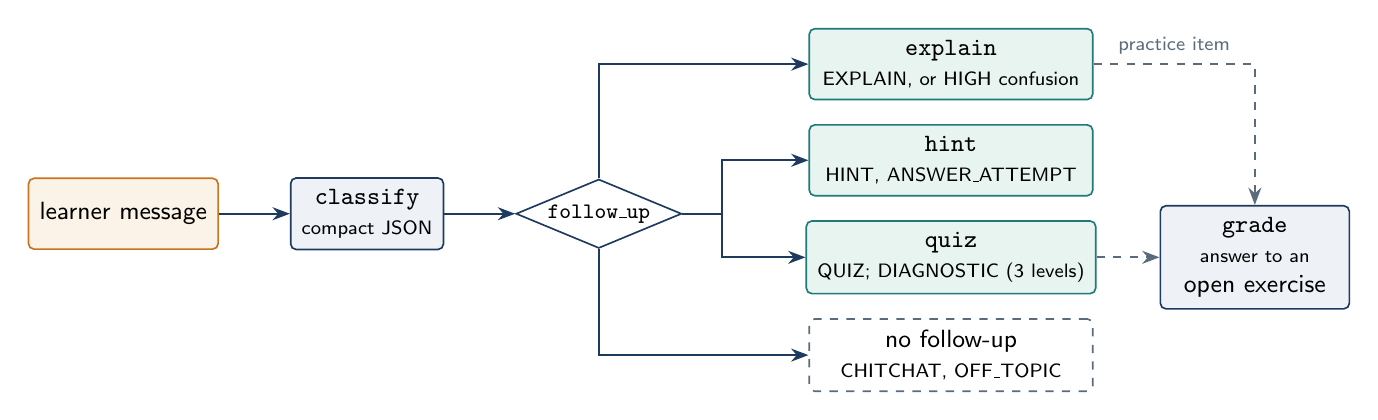
\begin{tikzpicture}[node distance=0.5cm and 0.9cm]
  \node[abox] (msg) {learner message};
  \node[box, right=of msg] (cls) {\texttt{classify}\\{\scriptsize compact JSON}};
  \node[dec, right=0.9cm of cls] (fu) {\texttt{follow\_up}};
  \node[tbox, right=1.6cm of fu, yshift=1.9cm, minimum width=3.6cm] (ex) {\texttt{explain}\\{\scriptsize EXPLAIN, or HIGH confusion}};
  \node[tbox, below=0.3cm of ex, minimum width=3.6cm] (hi) {\texttt{hint}\\{\scriptsize HINT, ANSWER\_ATTEMPT}};
  \node[tbox, below=0.3cm of hi, minimum width=3.6cm] (qz) {\texttt{quiz}\\{\scriptsize QUIZ; DIAGNOSTIC (3 levels)}};
  \node[gbox, below=0.3cm of qz, minimum width=3.6cm] (no) {no follow-up\\{\scriptsize CHITCHAT, OFF\_TOPIC}};
  \node[box, right=0.8cm of qz, minimum width=2.4cm] (gr) {\texttt{grade}\\\scriptsize answer to an\\open exercise};
  \draw[arr] (msg) -- (cls); \draw[arr] (cls) -- (fu);
  \draw[arr] (fu.north) |- (ex.west); \draw[arr] (fu.east) -- ++(0.5,0) |- (hi.west);
  \draw[arr] (fu.east) -- ++(0.5,0) |- (qz.west); \draw[arr] (fu.south) |- (no.west);
  \draw[darr] (qz.east) -- (gr.west);
  \draw[darr] (ex.east) -| node[lbl, above, pos=0.25]{practice item} (gr.north);
\end{tikzpicture}}
\caption{One learner turn, as \texttt{scripts/chat.py} implements it. Your feature layer owns this loop.}
\label{fig:turn}
\end{figure}

\subsection{hint}

\textbf{Inputs:} \texttt{problem} (required); \texttt{attempt}, \texttt{solution} (used only by the leak guard, never
sent as an answer); for bank exercises \texttt{stored\_hints} (list) + \texttt{hint\_level} (1-based).
\textbf{Output:} \texttt{text}, one guiding question (prompt asks ≤ 25 words).

With \texttt{stored\_hints}, the hint is served from the bank in order: 0 requests,
\texttt{data = \{hint\_level, hints\_total, source: "bank"\}}. Otherwise one compact call, then guards in order:
repetition loop → template; > 40 words → keep the leading complete question or template; solution
leaked (verbatim or as ``= value'') → template; wrong language → template; foreign Latin words in an
Arabic-script hint → flagged. Every guarded hint is \texttt{degraded} and never cached.

Real example: \texttt{problem="Calcule la dérivée de f(x) = 3x² + 5x"}, \texttt{attempt="6x"} → \textit{``Qu'est-ce qui
se passe lorsque tu multiplies la dérivée de 3x par 2, puis ajoutes 5 ?''} (compact, 4.0 s, 225/30 tokens).
Hint quality depends on the compact model; the guards only catch the unusable cases.

\subsection{explain}
\label{sec:explain}

\textbf{Inputs:} \texttt{question} (required); \texttt{history} (list of \texttt{\{"role","content"\}} turns, kept
newest-first within budget); \texttt{exclude\_exercises} (ids already served).
\textbf{Context:} \texttt{language}, \texttt{confusion}, \texttt{difficulty}, \texttt{escalate}/\texttt{complexity}, \texttt{topic}.

\textbf{Output:} \texttt{text} = opener + body + practice line; \texttt{data = \{body, opener, exercise\}}, where
\texttt{exercise = \{id, concept, level, statement, expression\}} (no solution, no hints). In fast mode:
\texttt{data = \{framing, excerpts: [\{chunk\_id, text\}], exercise\}} and \texttt{mode="fast\_extractive"}.

\begin{figure}[H]
\centering
\begin{tikzpicture}
  \node[abox, minimum width=10.5cm, anchor=west] (op) at (0,0) {\textbf{Opener}: template from \texttt{data/templates.yaml}, by language × confusion};
  \node[box, minimum width=10.5cm, minimum height=1.5cm, anchor=north west] (body) at ($(op.south west)+(0,-0.15)$) {\textbf{Body}: written by mid-size, in ONE language (French for FRENCH/DARIJA/ARABIZI,\\MSA for ARABIC, English for ENGLISH), ≤ 120 words, grounded in 2 course chunks.\\{\scriptsize This is the only part the model writes, and the only part cached.}};
  \node[tbox, minimum width=10.5cm, anchor=north west] (ex) at ($(body.south west)+(0,-0.15)$) {\textbf{Practice}: localized ``À toi :'' + first unserved bank exercise on the top chunk's concept};
  \draw[decorate,decoration={brace,amplitude=5pt,mirror},line width=0.6pt,color=slate] ($(op.north east)+(0.2,0)$) -- node[lbl,right=6pt,align=left]{deterministic} ($(op.south east)+(0.2,0)$);
  \draw[decorate,decoration={brace,amplitude=5pt,mirror},line width=0.6pt,color=amber] ($(body.north east)+(0.2,0)$) -- node[lbl,right=6pt,align=left,text=amber]{LLM, checked:\\formulas · loops\\language · words} ($(body.south east)+(0.2,0)$);
  \draw[decorate,decoration={brace,amplitude=5pt,mirror},line width=0.6pt,color=slate] ($(ex.north east)+(0.2,0)$) -- node[lbl,right=6pt,align=left]{deterministic} ($(ex.south east)+(0.2,0)$);
\end{tikzpicture}
\caption{Composition of an explain answer: narrow what the LLM writes, check what it does write.}
\label{fig:explain-composition}
\end{figure}

Outcomes you can get from explain:

\begin{tabularx}{\linewidth}{@{}L{5cm} Y@{}}
\toprule
\textbf{Situation} & \textbf{What the learner gets}\\
\midrule
normal & opener + mid-size body + exercise; cached for 7 days.\\
nothing in the course passes the gate & localized ``not in the course material'' text; 0 requests, not degraded, not cached.\\
mid-size busy, breaker open or quota low & \textbf{fast mode}: up to 5 course sentences verbatim + framing line + exercise; degraded, never cached.\\
body fails a check & text kept but \texttt{degraded} (\texttt{ungrounded\_formula}, \texttt{wrong\_math}, \texttt{language\_drift}, \texttt{contamination}); not cached; failed checks also set a negative marker.\\
body is a repetition loop & ≥ 40 good words before the loop → truncated text kept (\texttt{loop\_truncated}); otherwise fast mode (\texttt{degenerate}).\\
\bottomrule
\end{tabularx}

\subsection{grade}

\textbf{Inputs:} \texttt{problem}, \texttt{solution}, \texttt{attempt} (all required); \texttt{common\_mistakes} as a list
of dicts with keys \texttt{expr} and \texttt{feedback}, or of \texttt{[expr, feedback]} pairs.
\textbf{Output:} \texttt{data = \{verdict: CORRECT|INCORRECT|PARTIAL|UNKNOWN, mistake, feedback, graded\_by: "sympy"|"llm"\}}.

If both answer and solution parse as math (\texttt{x\textasciicircum{}2}, \texttt{x²}, \texttt{2x}, \texttt{x(x+3)}, \texttt{√x}, French decimal
commas, an \texttt{f'(x) =} prefix\dots), \texttt{sympy} decides by \texttt{simplify(a - b) == 0}: 0 requests. A wrong
answer equivalent to a stored mistake gets that mistake's feedback. Otherwise (sentences, text
solutions) one compact JSON call grades it; feedback that would leak the solution is blanked.
\texttt{UNKNOWN} is the safe default when the LLM grader fails.

Real example: \texttt{solution="f'(x) = 4x³"}, \texttt{attempt="x\textasciicircum{}3"}, mistake \texttt{"x³"} → \texttt{INCORRECT},
\texttt{mistake="x³"}, feedback from the bank, \texttt{graded\_by="sympy"}, 81 ms, 0 tokens.

\begin{warn}[Security]
\texttt{sympy}'s parser evaluates Python. Learner text is reduced to a whitelist (digits, \texttt{x}, operators,
brackets, \texttt{sqrt ln exp sin cos tan}; ≤ 80 characters) before parsing, and anything else goes to the
LLM grader. Keep that whitelist if you extend the math parser (\texttt{engine/mathcheck.py}).
\end{warn}

\subsection{quiz}

\textbf{Inputs (all optional):} \texttt{message} (the learner's request: its concepts are matched through the
glossary), \texttt{concept}, \texttt{difficulty} (1–3, nearest level is used), \texttt{exclude} (ids already served),
\texttt{diagnostic=True} (3 exercises: levels 1/2/3 on three concepts), \texttt{intro} (\texttt{True} = template,
\texttt{"llm"} = compact-written cached line, \texttt{False} = none).
\textbf{Output:} \texttt{text} (intro + statement), \texttt{data = \{exercises: [...], requested\_concepts,
diagnostic, intro\}}, \texttt{mode="bank"}. Always 0 requests unless \texttt{intro="llm"}.

To grade the learner's answer, look up the full exercise with \texttt{engine.exercises.get(id)} (it has
\texttt{solution}, \texttt{hints}, \texttt{common\_mistakes}) and call \texttt{grade} / \texttt{hint} with them, as
\texttt{scripts/chat.py} does.

\subsection{compress}

Used internally by explain when the retrieved chunks do not fit the prompt budget. Inputs:
\texttt{question}, \texttt{chunks}. The model sees numbered sentences and returns \texttt{\{"keep": [numbers]\}}, so it
cannot invent text (~10 output tokens). If that fails, a lexical pick is used. A chunk that loses
all its sentences gets its best one back: compression never drops a relevant chunk.

% ================================================================== 5
\section{Degrade reasons: the complete catalog}
\label{sec:degrade}

\begin{longtable}{@{}>{\ttfamily\small\raggedright\arraybackslash}p{4.1cm} >{\raggedright\arraybackslash}p{6.6cm} >{\small\raggedright\arraybackslash}p{4.6cm}@{}}
\toprule
\textrm{\textbf{degrade\_reason}} & \textbf{Meaning} & \textbf{Feature-layer suggestion}\\
\midrule
\endhead
quota\_low & local quota tokens < \texttt{QUOTA\_LOW\_THRESHOLD}: explain sent to fast mode proactively & show excerpts; offer full answer later\\
breaker\_open & mid-size had 3 saturations in 60 s: skipped for 30 s & same\\
midsize\_saturated & mid-size refused after retries: runtime fallback & same\\
service\_busy & every class saturated / concurrency refused (\texttt{eta\_seconds} set) & ``busy, retry in N s''\\
quota\_exhausted & stated quota delay longer than \texttt{MAX\_RETRY\_WAIT\_S} (BACKGROUND: \texttt{\_BACKGROUND}); \texttt{eta\_seconds} = the remaining block & same\\
input\_truncated & the provider cut the start of the prompt (\texttt{prompt\_tokens} far below the prompt size); never cached & show a fallback; shorten the input\\
service\_unavailable & transient 5xx/network errors exhausted (\texttt{eta\_seconds} set) & same\\
request\_too\_large & prompt cannot be trimmed under the ceiling & shorten history/input\\
provider\_error & other 4xx (bad key, unknown model\dots) & alert; check config\\
midsize\_unavailable & mid-size timed out or is down; \texttt{eta\_seconds} = when it is probed again (v1.2) & fast mode text is in the result\\
deadline & explain had no body after 25 s; the generation continues into the cache (v1.2) & fast mode text now; the next ask is a hit\\
superseded & the same learner queued a newer INTERACTIVE request (v1.3) & drop this result silently\\
room\_busy & another AI request of the room is running; \texttt{eta\_seconds} (v1.3) & disable the button, retry after the ETA\\
invalid\_image & \texttt{ocr\_transcribe}: not a readable image (v1.3) & ask for another photo\\
low\_confidence & \texttt{ocr\_transcribe}: text returned with visible reading problems (v1.3) & show with \texttt{confidence\_note}\\
json\_invalid & \texttt{check\_claim}: no valid JSON after the repair call (v1.3) & treat the verdict as unknown\\
\midrule
ungrounded\_formula & a formula neither verifiable nor in the sources & show; mark ``check with teacher''\\
wrong\_math & a derivative/identity claim sympy proves false & consider hiding the body\\
explain\_guard:loop\_truncated & repetition loop cut after the last full sentence & show\\
explain\_guard:degenerate / :empty & unusable output: served in fast mode & show excerpts\\
explain\_guard:language\_drift & body in the wrong script & show; maybe retry later\\
explain\_guard:contamination & foreign Latin words in an Arabic-script answer & show\\
hint\_guard:degenerate / :too\_long / :answer\_leak / :language\_drift & hint replaced by a safe template & show (the template is fine)\\
hint\_guard:contamination & flagged words, text kept & show\\
\bottomrule
\end{longtable}

\textbf{Degraded results are never cached.} The deterministic-check failures
(\texttt{ungrounded\_formula}, \texttt{wrong\_math}, \texttt{loop\_truncated}, \texttt{degenerate}) also set a
\textbf{negative marker} so that the same question within 10 minutes does not burn another identical
request (§\ref{sec:cache}).

% ================================================================== 6
\section{Inside \texttt{engine.run}: the request lifecycle}
\label{sec:lifecycle}

\begin{figure}[H]
\centering
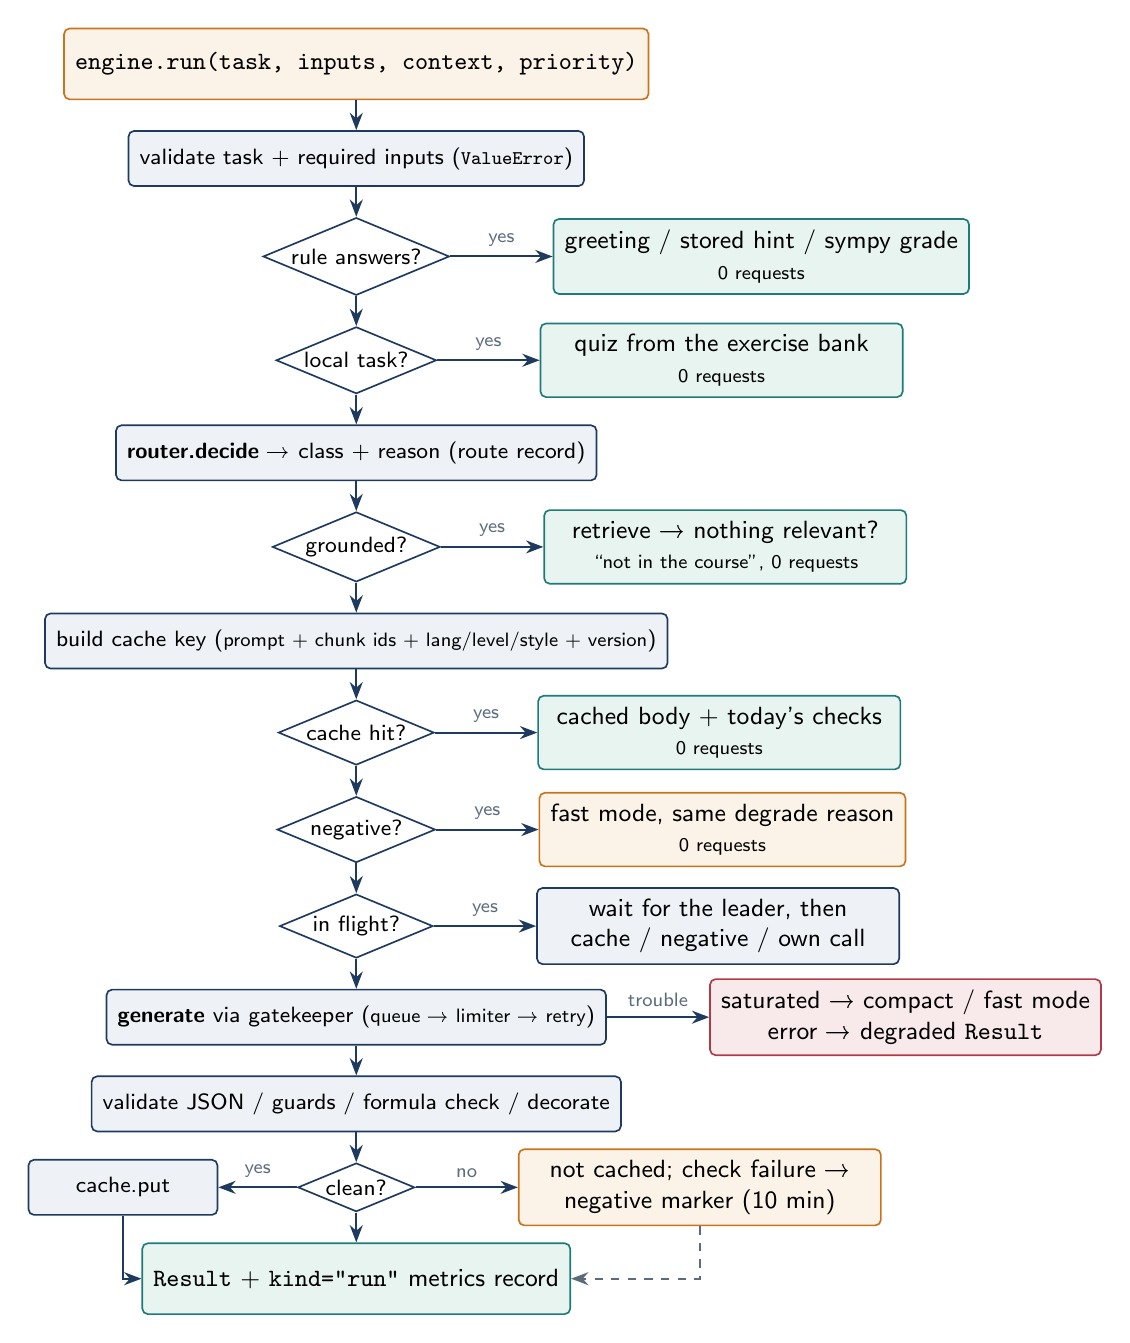
\begin{tikzpicture}[node distance=0.38cm, every node/.append style={font=\sffamily\footnotesize}]
  \node[abox, minimum width=5.2cm] (s) {\texttt{engine.run(task, inputs, context, priority)}};
  \node[sbox, below=of s, minimum width=5.2cm] (v) {validate task + required inputs ({\scriptsize\texttt{ValueError}})};
  \node[dec, below=of v] (sc) {rule answers?};
  \node[dec, below=of sc] (lc) {local task?};
  \node[sbox, below=of lc, minimum width=5.2cm] (rt) {\textbf{router.decide} → class + reason (route record)};
  \node[dec, below=of rt] (gr) {grounded?};
  \node[sbox, below=of gr, minimum width=5.2cm] (key) {build cache key ({\scriptsize prompt + chunk ids + lang/level/style + version})};
  \node[dec, below=of key] (hit) {cache hit?};
  \node[dec, below=of hit] (neg) {negative?};
  \node[dec, below=of neg] (inf) {in flight?};
  \node[sbox, below=of inf, minimum width=5.2cm] (gen) {\textbf{generate} via gatekeeper ({\scriptsize queue → limiter → retry})};
  \node[sbox, below=of gen, minimum width=5.2cm] (chk) {validate JSON / guards / formula check / decorate};
  \node[dec, below=of chk] (cl) {clean?};
  \node[tbox, below=of cl, minimum width=5.2cm] (fin) {\texttt{Result} + \texttt{kind="run"} metrics record};
  % right side outcomes
  \node[tbox, right=1.3cm of sc, minimum width=4.6cm] (o1) {greeting / stored hint / sympy grade\\{\scriptsize 0 requests}};
  \node[tbox, right=1.3cm of lc, minimum width=4.6cm] (o2) {quiz from the exercise bank\\{\scriptsize 0 requests}};
  \node[tbox, right=1.3cm of gr, minimum width=4.6cm] (o3) {retrieve → nothing relevant?\\{\scriptsize ``not in the course'', 0 requests}};
  \node[tbox, right=1.3cm of hit, minimum width=4.6cm] (o4) {cached body + today's checks\\{\scriptsize 0 requests}};
  \node[abox, right=1.3cm of neg, minimum width=4.6cm] (o5) {fast mode, same degrade reason\\{\scriptsize 0 requests}};
  \node[box, right=1.3cm of inf, minimum width=4.6cm] (o6) {wait for the leader, then\\cache / negative / own call};
  \node[rbox, right=1.3cm of gen, minimum width=4.6cm] (o7) {saturated → compact / fast mode\\error → degraded \texttt{Result}};
  \node[abox, right=1.3cm of cl, minimum width=4.6cm] (o8) {not cached; check failure →\\negative marker (10 min)};
  \node[sbox, left=1.0cm of cl, minimum width=2.4cm] (put) {cache.put};
  \foreach \a/\b in {s/v,v/sc,sc/lc,lc/rt,rt/gr,gr/key,key/hit,hit/neg,neg/inf,inf/gen,gen/chk,chk/cl,cl/fin} \draw[arr] (\a) -- (\b);
  \foreach \a/\b in {sc/o1,lc/o2,gr/o3,hit/o4,neg/o5,inf/o6} \draw[arr] (\a) -- node[lbl,above]{yes} (\b);
  \draw[arr] (gen) -- node[lbl,above]{trouble} (o7);
  \draw[arr] (cl) -- node[lbl,above]{no} (o8);
  \draw[arr] (cl) -- node[lbl,above]{yes} (put);
  \draw[arr] (put) |- (fin);
  \draw[darr] (o8.south) |- (fin.east);
\end{tikzpicture}
\caption{What \texttt{engine.run} does, in order (\texttt{engine/core.py}). Every right-hand exit ends in the same \texttt{Result} shape.}
\label{fig:lifecycle}
\end{figure}

Two details matter when you modify the flow:

\begin{itemize}
  \item \textbf{The cache key uses the router's preferred class}, not the class actually used. A request
  moved to compact by low quota can still be served a cached mid-size answer, which is better than a
  fresh compact one.
  \item \textbf{For explain, the key is built from the chunk ids}, not from the compressed text, so the
  lookup happens before compression and a hit costs nothing, compression included.
\end{itemize}

% ================================================================== 7
\section{Gatekeeper: living inside the platform limits}
\label{sec:gatekeeper}

Every LLM and embedding request goes through \texttt{gatekeeper/}. Nothing else talks to the provider;
this is what makes the metrics trustworthy.

\begin{figure}[H]
\centering
\begin{tikzpicture}[node distance=0.55cm]
  \node[box, minimum width=2.4cm, minimum height=1.4cm] (q) {\textbf{Priority queue}\\\scriptsize INTERACTIVE ≺\\BACKGROUND, FIFO};
  \node[box, right=of q, minimum width=2.6cm, minimum height=1.4cm] (b) {\textbf{Sliding window}\\\scriptsize 20 per 60 s\\any rolling minute};
  \node[box, right=of b, minimum width=2.4cm, minimum height=1.4cm] (sem) {\textbf{Semaphore}\\\scriptsize max 2\\in flight};
  \node[box, right=of sem, minimum width=2.2cm, minimum height=1.4cm] (c) {\textbf{Client}\\\scriptsize POST\\/chat/completions};
  \node[rbox, right=of c, minimum width=1.9cm, minimum height=1.4cm] (p) {\textbf{Provider}};
  \node[abox, below=1.1cm of sem, minimum width=4.6cm] (e) {\texttt{errors.classify\_response}\\{\scriptsize status + body + headers → typed error}};
  \node[abox, left=0.9cm of e, minimum width=3.6cm] (r) {\texttt{retry.\_decide}\\{\scriptsize one action per error}};
  \node[tbox, above=0.7cm of b, minimum width=5.6cm] (h) {quota headers on 200 → phantom entries, never above server};
  \draw[arr] (q) -- (b); \draw[arr] (b) -- (sem); \draw[arr] (sem) -- (c); \draw[arr] (c) -- (p);
  \draw[arr] (p.south) |- (e.east);
  \draw[arr] (e) -- (r);
  \draw[arr] (r.west) -| node[lbl, left, pos=0.8, align=right]{retry, same\\queue position} (q.south);
  \draw[darr] (p.north) |- (h.east);
  \draw[darr] (h.south) -- (b.north);
\end{tikzpicture}
\caption{The gatekeeper path of one attempt. Quota waits happen in the window and never hold a concurrency slot.}
\label{fig:gatekeeper}
\end{figure}

\subsection{Rate and concurrency are two mechanisms}

\begin{itemize}
  \item \textbf{Sliding window} (rate): a log of send times; at most \texttt{RATE\_LIMIT\_PER\_MIN} (20) sends in
  any rolling \texttt{RATE\_WINDOW\_S} (60) seconds. FelCloud keeps the key closed for the full minute after the
  21st request, so a bucket with a burst reserve overshoots it. Embeddings have their own window (60/min),
  because the platform has a separate embeddings quota.
  \item \textbf{Semaphore} (concurrency): at most \texttt{MAX\_CONCURRENT} (2) requests in flight, shared by
  chat and embeddings (assumed per key).
  \item A request waits for a free window slot \emph{before} taking a concurrency slot, and records its send only once
  it has the slot. So a quota wait never blocks a slot, and requests queued on the semaphore cannot
  burst past the window.
  \item \textbf{Server feedback}: \texttt{x-ratelimit-api\_key-remaining-requests} on every 200 adds phantom
  entries when it is below the local free count, so local never exceeds the server; a stated quota delay blocks the window until it expires.
\end{itemize}

\subsection{Priority queue}

One dispatcher per kind (chat, embeddings) waits until the limiter has capacity and only
\emph{then} pops the best waiter. Choosing at grant time is what lets an interactive request that
arrives behind 50 background ones leave first. A retry keeps its original sequence number, so a
request that waited out a quota delay is not sent to the back. The queue also keeps a moving average
of how long requests hold a slot, which gives the \texttt{eta\_s} of \texttt{queued} events and of busy results:

\[
  \text{eta} \;=\; \text{Retry-After} \;+\; \frac{(\text{queue depth} + 1)\times \overline{t_{\text{slot}}}}{\texttt{MAX\_CONCURRENT}}
\]

\subsection{The platform contract as code}
\label{sec:retry}

\begin{table}[H]
\centering\small
\begin{tabularx}{\linewidth}{@{}L{4.0cm} T{3.1cm} Y T{2.9cm}@{}}
\toprule
\textbf{Provider says} & \textbf{Typed error} & \textbf{Action} & \textbf{Event}\\
\midrule
429 quota (\texttt{rate\_limit\_type: requests}, \texttt{retry-after: 60}; any 429 that is not cooldown/concurrency) & \texttt{QuotaExhausted} & delay = the \texttt{retry-after} header only; the window is blocked until it expires; BACKGROUND waits up to 65 s, INTERACTIVE up to 30 s, otherwise give up with \texttt{eta} = the remaining block; never hop models (the quota is per key) & \texttt{wait\_stated\_delay}\\
503 + Retry-After, or LiteLLM 429 \texttt{all\_deployments\_in\_cooldown} & \texttt{ModelSaturated} & mid-size: retry once, then the router falls back. compact: up to 3 retries & \texttt{retry\_after\_interval}\\
429 parallel/concurrent (\texttt{rate\_limit\_type: max\_parallel\_requests}) & \texttt{ConcurrencyLimited} & wait \texttt{min(Retry-After, CONCURRENCY\_RETRY\_WAIT\_S)} = 2 s (it states 60 s) & \texttt{wait\_slot}\\
400 naming a ceiling & \texttt{CeilingExceeded} & fix once (trim \texttt{max\_tokens} or the longest message), retry once & \texttt{fix\_request}\\
5xx, network, timeout & \texttt{TransientError} & exponential backoff + full jitter (only when no delay is stated) & \texttt{backoff}\\
other 4xx & \texttt{FatalError} & give up immediately & \texttt{gave\_up}\\
200 & — & read quota headers, pace & —\\
\bottomrule
\end{tabularx}
\caption{\texttt{gatekeeper/errors.py} (mapping) and \texttt{gatekeeper/retry.py} (actions). At most \texttt{MAX\_ATTEMPTS}=4 attempts.}
\end{table}

\begin{note}[What was observed on the real FelCloud (recon, 22 Oct)]
FelCloud is a LiteLLM proxy behind Caddy (server timeout 90 s → client timeout 85 s). Saturation
arrived as \textbf{429 \texttt{all\_deployments\_in\_cooldown}} with \texttt{Retry-After: 5}, not the annex's
503, so both are mapped to \texttt{ModelSaturated}. There was \textbf{no 400 for long prompts}: input was
\textbf{silently truncated near 2048 tokens}. The client therefore enforces its own input budget
(\texttt{INPUT\_TOKEN\_BUDGET}=1800 then) and trims \emph{before} sending.
\end{note}

\begin{note}[Updated by the probes of 26 Oct (engine v1.1)]
Both 429 refusals were observed: status 429, \texttt{retry-after: 60}, \texttt{rate\_limit\_type} \texttt{requests} or \texttt{max\_parallel\_requests}; \texttt{Limit resets at} in the body is the refusal time plus 60 s and is ignored. Both are \texttt{CONFIRMED(felcloud)} in \texttt{errors.py}, with the real responses as test fixtures. The input window is about \textbf{4,096 tokens}, and overflow silently drops the \emph{start} of the prompt, so the engine checks estimated prompt + output cap against \texttt{CONTEXT\_WINDOW} × 0.85, estimates at 2.3 characters per token (Arabizi, the worst measured case), raises \texttt{INPUT\_TOKEN\_BUDGET} to 2800, and degrades any answer whose \texttt{prompt\_tokens} shows the input was cut (\texttt{input\_truncated}). \texttt{max\_tokens} is ignored; only a top-level \texttt{options.num\_predict} caps the output, and \texttt{finish\_reason} stays \texttt{stop} when it cuts, so \texttt{completion\_tokens} $\ge$ cap means cut.
\end{note}

% ================================================================== 8
\section{Router: compact first, mid-size by rule}

\texttt{router/policy.py} holds the routing table (\texttt{ROUTES}) and every routing decision; each one is
logged as a \texttt{kind="route"} metrics record with its reason.

\begin{lstlisting}
ROUTES = {"classify": Route(C), "hint": Route(C), "grade": Route(C),
          "compress": Route(C), "summary": Route(C), "quiz": Route(C),
          "explain": Route(M, fallback=C)}
\end{lstlisting}

For explain the decision is, in order:
\begin{enumerate}
  \item default mid-size;
  \item if local quota tokens < \texttt{QUOTA\_LOW\_THRESHOLD} (2) and the call is \textbf{not escalated}
  (\texttt{escalate=True} or \texttt{complexity >= 4}) → compact, \texttt{degraded}, reason \texttt{quota\_low};
  \item if the mid-size circuit breaker is open → compact, reason \texttt{breaker\_open} (escalation does not
  bypass it: escalating cannot help a class that is down);
  \item at run time, if mid-size stays saturated after its retry → \texttt{midsize\_saturated} fallback.
\end{enumerate}
For explain, ``compact'' means \textbf{fast mode}: compact does not write the explanation (it misquoted
the course in tests); the learner gets verbatim course sentences plus one framing line.

\begin{figure}[H]
\centering
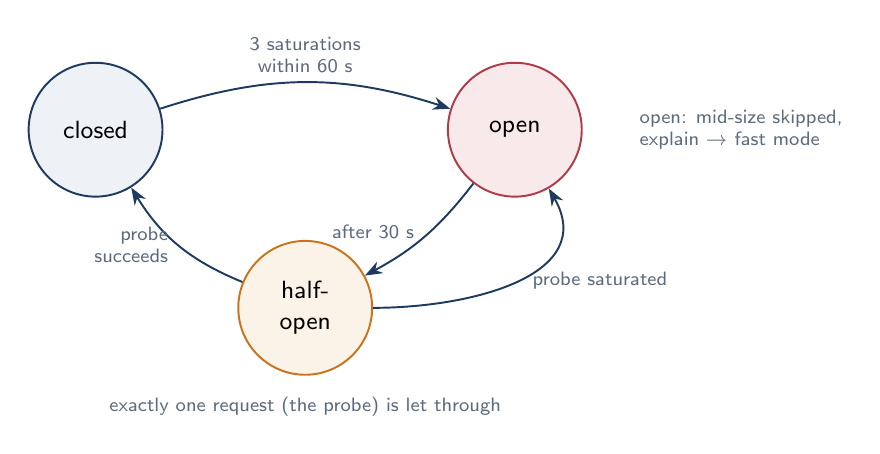
\begin{tikzpicture}[node distance=2.6cm, state/.style={circle, draw=navy, fill=mist, line width=0.7pt, minimum size=1.7cm, align=center, font=\sffamily\small}]
  \node[state] (cl) {closed};
  \node[state, draw=rose, fill=blush, right=3.6cm of cl] (op) {open};
  \node[state, draw=amber, fill=sand, below=1.4cm of $(cl)!0.5!(op)$] (ho) {half-\\open};
  \draw[arr] (cl) to[bend left=18] node[lbl, above, align=center]{3 saturations\\within 60 s} (op);
  \draw[arr] (op) to[bend left=12] node[lbl, left=2pt, pos=0.45]{after 30 s} (ho);
  \draw[arr] (ho) to[bend left=18] node[lbl, left, align=right]{probe\\succeeds} (cl);
  \draw[arr] (ho) to[out=0, in=-60, looseness=1.2] node[lbl, right=2pt, pos=0.5]{probe saturated} (op);
  \node[lbl, align=left, right=0.6cm of op] {open: mid-size skipped,\\explain → fast mode};
  \node[lbl, align=left, below=0.15cm of ho] {exactly one request (the probe) is let through};
\end{tikzpicture}
\caption{Mid-size circuit breaker (\texttt{router/breaker.py}). Only saturation responses count; quota refusals are per key and say nothing about class load.}
\label{fig:breaker}
\end{figure}

A probe that never reaches mid-size (cache hit, not found, fast path) releases its slot at the end of
\texttt{engine.run}; a probe that never reports expires after one cooldown, so the breaker cannot stay stuck
half-open.

% ================================================================== 9
\section{Caching and deduplication}
\label{sec:cache}

\begin{figure}[H]
\centering
\resizebox{\linewidth}{!}{%
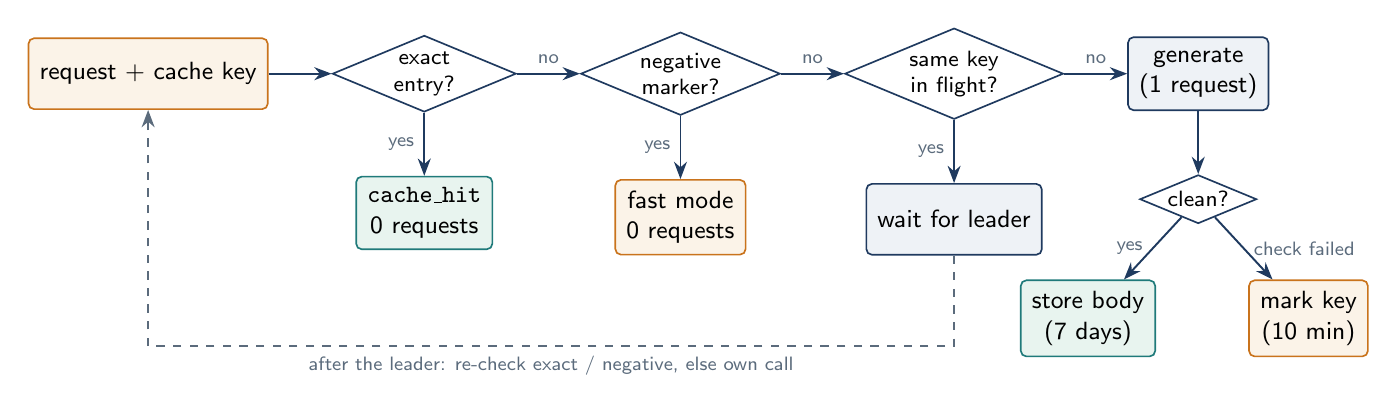
\begin{tikzpicture}[node distance=0.5cm and 0.8cm]
  \node[abox] (req) {request + cache key};
  \node[dec, right=of req] (ex) {exact\\entry?};
  \node[dec, right=of ex] (ng) {negative\\marker?};
  \node[dec, right=of ng] (fl) {same key\\in flight?};
  \node[box, right=of fl] (gen) {generate\\(1 request)};
  \node[tbox, below=0.8cm of ex] (h) {\texttt{cache\_hit}\\0 requests};
  \node[abox, below=0.8cm of ng] (n) {fast mode\\0 requests};
  \node[box, below=0.8cm of fl] (w) {wait for leader};
  \node[dec, below=0.8cm of gen] (ok) {clean?};
  \node[tbox, below=0.7cm of ok, xshift=-1.4cm] (put) {store body\\(7 days)};
  \node[abox, below=0.7cm of ok, xshift=1.4cm] (mark) {mark key\\(10 min)};
  \draw[arr] (req) -- (ex); \draw[arr] (ex) -- node[lbl,above]{no} (ng); \draw[arr] (ng) -- node[lbl,above]{no} (fl);
  \draw[arr] (fl) -- node[lbl,above]{no} (gen);
  \draw[arr] (ex) -- node[lbl,left]{yes} (h); \draw[arr] (ng) -- node[lbl,left]{yes} (n); \draw[arr] (fl) -- node[lbl,left]{yes} (w);
  \draw[arr] (gen) -- (ok);
  \draw[arr] (ok) -- node[lbl,left]{yes} (put); \draw[arr] (ok) -- node[lbl,right]{check failed} (mark);
  \draw[darr] (w.south) -- ++(0,-1.15) -| node[lbl,below,pos=0.25]{after the leader: re-check exact / negative, else own call} (req.south);
\end{tikzpicture}}
\caption{Three ways the engine avoids a repeated identical request.}
\end{figure}

\begin{itemize}
  \item \textbf{Exact cache} (SQLite, \texttt{CACHE\_TTL\_DAYS}=7). Key = SHA-256 of task, preferred class,
  normalized prompt (whitespace collapsed, Unicode NFC, \emph{no} lower-casing: \texttt{X} ≠ \texttt{x} in
  math), language, level, style, prompt-file version, and for explain the retrieved chunk ids.
  Editing a prompt bumps its version and invalidates its old answers automatically.
  \item \textbf{Only clean results are stored}: \texttt{put()} itself refuses degraded, fallback and
  safe-default values. Cache hits re-run today's deterministic checks (an explain entry that now
  fails is deleted; classify re-applies its rules).
  \item \textbf{Coalescing}: a request whose key is already being generated waits for the leader and
  is then served from the cache (\texttt{waiting\_identical\_request} → \texttt{cache\_hit}).
  \item \textbf{Negative cache} (\texttt{NEGATIVE\_CACHE\_TTL\_S}=600, 0 = off): an explain answer that failed
  a deterministic check marks its key. A repeat within the TTL gets fast mode with the same degrade
  reason and \textbf{0 requests}, logged as \texttt{outcome="negative\_cache\_hit"},
  \texttt{from\_negative\_cache=true}. Transient failures (saturation, quota) are never marked.
  \item \textbf{No semantic cache}: it was specified for explain, but FelCloud exposes no embedding
  model, so it was not built (§\ref{sec:improve}).
\end{itemize}

% ================================================================== 10
\section{Retrieval (RAG) for explain}
\label{sec:rag}

\begin{figure}[H]
\centering
\begin{tikzpicture}[node distance=0.42cm]
  \node[abox, minimum width=2.1cm] (q) {question};
  \node[sbox, right=of q, minimum width=2.4cm] (t) {normalize +\\tokenize};
  \node[sbox, right=of t, minimum width=2.3cm] (g) {glossary\\expansion};
  \node[sbox, right=of g, minimum width=2.4cm] (b) {BM25 per\\language plan};
  \node[sbox, right=of b, minimum width=2.3cm] (c) {coverage\\gate ≥ 0.4};
  \node[tbox, right=of c, minimum width=1.6cm] (k) {top 2\\chunks};
  \node[sbox, below=0.9cm of b, minimum width=4.6cm] (bud) {budget assembly (≤ 1620 est. tokens)\\system + question → chunks → history};
  \node[sbox, left=0.7cm of bud, minimum width=3.4cm] (cmp) {extractive compress\\only if chunks don't fit};
  \node[box, right=0.7cm of bud, minimum width=2.6cm] (m) {mid-size\\prompt};
  \draw[arr] (q) -- (t); \draw[arr] (t) -- (g); \draw[arr] (g) -- (b); \draw[arr] (b) -- (c); \draw[arr] (c) -- (k);
  \draw[arr] (k.south) |- ($(bud.north)+(0,0.35)$) -- (bud.north);
  \draw[darr] (bud.west) -- (cmp.east);
  \draw[arr] (bud.east) -- (m.west);
  \draw[darr] (c.north) -- ++(0,0.5) node[lbl, above]{nothing passes → ``not in the course'', 0 requests};
\end{tikzpicture}
\caption{Retrieval pipeline. No embeddings and no model call: BM25 in pure Python.}
\label{fig:rag}
\end{figure}

\begin{description}[style=nextline, leftmargin=0.6cm, font=\sffamily\bfseries\color{navy}]
  \item[Course documents] \texttt{data/docs/*.md}, one file per topic and language, with a front matter
  (\texttt{topic}, \texttt{level}, \texttt{language}, \texttt{title}, optional \texttt{status: draft}) and \texttt{\#\#} sections
  of about 250–300 tokens, each tagged \texttt{<!-{}- concept: id -{}->}. \texttt{python -m scripts.index\_docs}
  writes \texttt{data/index/chunks.json}; chunk id = \texttt{<file stem>\#<section slug>}, stable across
  re-indexing. Drafts are skipped until reviewed.
  \item[Tokenization] NFKC (\texttt{x²} → \texttt{x2}); Arabic diacritics/tatweel stripped and letters normalized
  before splitting; accent folding and light plural/\textit{e} stemming on Latin words only
  (\texttt{dérivée}, \texttt{derivee}, \texttt{dérivés} → \texttt{deriv}); Arabic prefix stripping; FR/EN/Arabizi/Arabic stopwords.
  \item[Glossary] \texttt{data/glossary.yaml} maps 327 learner variants (Darija, Arabizi, MSA, English) to 60
  French course terms, deterministically. Course terms are weighted 0.5 so the learner's own words
  dominate. This is what lets ``mochtaqa'' or an Arabic-script question find a French chunk.
  \item[Relevance gate] \emph{coverage}, not BM25 score: the IDF-weighted share of the question's
  concepts found in the chunk. On a one-topic corpus raw scores fail (``the function in my code is
  slow'' outscored a real question). Measured: on-topic ≥ 0.49, off-topic ≤ 0.28 → threshold 0.4.
  \item[Language plan] DARIJA/ARABIZI → French chunks; ARABIC → Arabic, else French; ENGLISH →
  English, else French; FRENCH → all.
  \item[Budget] prompts are assembled within \texttt{INPUT\_TOKEN\_BUDGET × (1 − 0.1)} = 1620 estimated
  tokens; history is dropped oldest-first without gaps; everything dropped is listed in \texttt{notes.dropped}.
\end{description}

\begin{idea}[Swap the retriever]
\texttt{RETRIEVER=embedding} selects \texttt{EmbeddingRetriever} (cosine over gatekeeper embeddings, using
the separate embeddings quota). Any object with \texttt{async index(chunks)} and
\texttt{async search(question, k, filters, expansion) -> list[Hit]} can be passed to \texttt{Engine.create(retriever=...)}.
\end{idea}

% ================================================================== 11
\section{The deterministic layer}

The design principle: \textbf{narrow what the LLM writes, and check what it does write.} Small models
on CPU are slow and unreliable; every sentence a rule or a template can produce is a request saved
and a failure avoided.

\begin{tabularx}{\linewidth}{@{}L{4.4cm} Y@{}}
\toprule
\textbf{Mechanism} & \textbf{What it does}\\
\midrule
Templates (\texttt{data/templates.yaml}) & openers by language × confusion, ``your turn'' lines, fast-mode framing and quiz intros (Darija/Arabizi always from templates), generic grading feedback.\\
Exercise bank (\texttt{data/exercises/*.yaml}) & 15 exercises, 11 concepts, levels 1–3, each with 3 graded hints and common mistakes; statements rendered in FR/EN/AR from phrase templates.\\
Formula check (\texttt{engine/grounding.py}) & every ``A = B'' and every formula-like run in an explain body is \emph{verified} (sympy: \texttt{f'(x) = D} against the answer's own \texttt{f(x) = E}, values, identities), \emph{skipped} (assignments like \texttt{n = 2}, equations to solve, refuted claims after ``not''), or else must appear in the sources. False → \texttt{wrong\_math}; neither → \texttt{ungrounded\_formula}.\\
Loop detection (\texttt{engine/tasks.py}) & a 3-word phrase recurring 3+ times in a row, each within 12 words: salvage the text before it if ≥ 40 words and ending on a full sentence.\\
Language checks & classify's language reconciled with script and Tunisian markers; explain/hint drift guards; Latin-word contamination in Arabic-script answers.\\
\bottomrule
\end{tabularx}

% ================================================================== 12
\section{Metrics: what is measured}

Every provider attempt, routing decision, breaker change, cache hit and engine call writes one
\texttt{CallRecord} (\texttt{metrics/record.py}) to \texttt{METRICS\_PATH} (JSONL).

\begin{tabularx}{\linewidth}{@{}T{5.2cm} Y@{}}
\toprule
\textrm{\textbf{Field}} & \textbf{Meaning}\\
\midrule
kind & \texttt{chat} / \texttt{embed} (one attempt or cache hit), \texttt{route}, \texttt{run}, \texttt{breaker}\\
request\_id, turn\_id, attempt & one engine call (shared by its retries) / one learner turn / attempt number\\
task, priority, purpose & task name; INTERACTIVE/BACKGROUND; \texttt{repair}, \texttt{framing} for side calls\\
model\_class, model & what was called\\
request\_hash & hash of the full request body: the same hash twice = repeated identical request\\
status, outcome, action & HTTP status; \texttt{ok}, \texttt{quota\_exhausted}, \texttt{saturated}, \texttt{cache\_hit}, \texttt{negative\_cache\_hit}\dots; what was done about it\\
wait\_ms, latency\_ms & time waiting (limiter, delays) / provider time\\
tokens\_in, tokens\_out, quota\_remaining & usage and the quota header\\
from\_cache, from\_negative\_cache, degraded, degrade\_reason, mode, graded\_by, eta\_s, detail & run outcome details; \texttt{detail} = route reason or provider message (never secrets)\\
\bottomrule
\end{tabularx}

\begin{lstlisting}[style=plain]
python -m scripts.load_test --sim-profile normal --n 50       # also: saturated, quota_low, capacity
python -m scripts.metrics_report metrics/load_normal.jsonl metrics/load_saturated.jsonl --out reports/x
\end{lstlisting}

The report gives, side by side: provider requests, calls per model, compact/mid-size split, tokens,
cache hit rate, repeated identical requests, refusals and how each was handled, degradations,
breaker trips, latency percentiles per task and priority, and a per-turn capacity estimate.


% ================================================================== v1.3
\section{What is new in v1.3}
\label{sec:v13}

v1.3 makes the engine ready for every Phase 1 feature of the team's contracts document. The public interface is unchanged
(\texttt{engine.run}, \texttt{Result}, \texttt{Event}); everything below is additive. The contract the feature layer
codes against is \texttt{docs/ENGINE\_API.md}: every task, its inputs and outputs, events, degrade reasons, request cost and a
JSON example per outcome. It is generated from the engine's real output (\texttt{python -m scripts.gen\_api\_examples --doc}),
and a test fails when it drifts from the code. Until the real engine is wired, \texttt{engine.fake.FakeEngine} has the same
\texttt{run} signature and returns the same shapes, events and timings in three modes (normal, slow, degraded), with
\texttt{context["fake\_outcome"]} to force one state, so the UIs can show every state without any LLM.

\subsection{Identity, fairness and the background reserve}

\begin{itemize}[leftmargin=1.4em,itemsep=2pt]
\item \textbf{Ids.} \texttt{learner\_id}, \texttt{room\_id}, \texttt{course\_id} and \texttt{class\_id} in the context are copied into
every metrics record of the run (ids only, never names), also those of helper runs and of the generation that outlives an
interactive deadline. They are not part of any cache key.
\item \textbf{One waiting request per learner.} A newer INTERACTIVE request of the same learner replaces the older one while it
still waits in the queue; the older returns at once, degraded \texttt{superseded}, nothing sent. A request already running is
never touched; BACKGROUND work is not limited.
\item \textbf{One request per room.} A second \texttt{run} with the same \texttt{room\_id} while one is in flight returns
\texttt{room\_busy} with an \texttt{eta\_seconds} (an average of the room's recent run times, minus the time already spent).
Helper runs (the grade call inside \texttt{check\_answer}) keep the learner's ids but not the room.
\item \textbf{Background reserve.} A BACKGROUND chat request is not granted while fewer than \texttt{BACKGROUND\_RESERVE} (6)
sends remain in the 20-per-minute window; it waits for entries to expire and announces it once (event \texttt{waiting\_reserve}).
A prep plan or an ingest can therefore never use the window a learner is about to need. Interactive requests ignore the reserve.
\end{itemize}

\subsection{The vision class}

\texttt{ModelClass.VISION} (\texttt{MODEL\_VISION}, default \texttt{deepseek-ocr}) reads images. The client sends OpenAI content parts
(an \texttt{image\_url} with a base64 data URL); the engine decodes, orients and resizes every image to at most one megapixel and
counts its estimated tokens in the input budget (a request that cannot fit is refused locally, nothing sent). Vision has its own
timeout (\texttt{TIMEOUT\_VISION\_S}, 40 s) and, like mid-size, is never retried after a hang. It shares the chat rate window and the
two concurrency slots with the other classes until the organizers say otherwise; mid-size and vision together may hold at most
\texttt{MAX\_CONCURRENT}$-1$ slots, so compact work always has one (an interactive photo can therefore wait behind a mid-size generation that is still running into the cache; its \texttt{queued} event carries an ETA). A learner's explain is bounded by the 25 s deadline in every path, also while it waits for an identical request that another learner or a prep page is generating. Whether a vision request really counts in the 20-per-minute
window is measured by \texttt{scripts/load\_mixed --real --probe-vision} (not yet run: no slot).

\subsection{New tasks}

\begin{tabularx}{\linewidth}{@{}>{\ttfamily\small}p{2.9cm} >{\small}p{2.2cm} >{\small}p{2.4cm} Y@{}}
\toprule
\textrm{\textbf{task}} & \textbf{class} & \textbf{requests} & \textbf{what it does}\\
\midrule
ocr\_transcribe & vision & 1 (0 cached) & photo of work $\to$ \{text, latex, confidence\_note\}; never grades; cache by image content\\
check\_claim & rules, compact & 0 or 1 & is this claim true in the course: sympy for formulas, retrieval gate (\texttt{NOT\_IN\_COURSE}), else one JSON call\\
check\_answer & rules, compact & 0 to 2 & a worked solution line by line: OK, WRONG or UNCHECKED; stored mistakes, buggy rules, guarded guiding question; the last line through grade\\
prep\_plan & none & 0 & study plan: prerequisites first, lowest mastery next, spread at the learner's pace, mastered concepts reviewed\\
generate\_page & mid-size & 0 or 1 & a prep page: explain at BACKGROUND through the tutor's cache, a bank worked example, three quiz items (variants fill gaps)\\
\bottomrule
\end{tabularx}

\medskip\noindent Three rules that run through them: a line or text that cannot be parsed is \texttt{UNCHECKED}, never \texttt{WRONG};
a guiding question is checked so it never states the answer (the hint guard plus the true derivative written out); and a
verdict that sympy can compute is never left to a model. \texttt{check\_claim} decides in this order: a refuted formula is
\texttt{CONTRADICTED} with the correct form (half refuted, half verified: \texttt{PARTLY}); a verified formula with no other
claim around it is \texttt{SUPPORTED}; anything else goes to retrieval, whose gate gives \texttt{NOT\_IN\_COURSE} at no cost, and
only then to one compact JSON call with the repair ladder and a degraded \texttt{PARTLY} as the safe default.
\texttt{explain} gains two inputs: \texttt{passage} (the text a learner selected: in the prompt, and retrieval runs on it first)
and \texttt{board\_text} (whiteboard text, trimmed to a share of the budget); both are in the cache key by a hash of the full text.

\subsection{Course content}

A course is a graph (\texttt{data/courses/<course>.yaml}: units with order and prerequisites, concepts with prerequisites and related
concepts, titles in French, English and Arabic). Concept ids are those of the exercise bank and of the \texttt{<!-- concept: id -->}
tags of the course documents, and a test checks the three agree in both directions and that \texttt{requires} has no cycle.
The retriever can add and remove chunks at runtime (\texttt{Engine.add\_material}, \texttt{remove\_material}), persists them per
course, and filters by \texttt{course\_id} plus visibility: public course documents, class material for that \texttt{class\_id},
private uploads for that \texttt{learner\_id}; a viewer without an id never sees class or private material. Professor material
has its BM25 score multiplied by \texttt{SOURCE\_BOOST\_PROFESSOR} and wins ties; the coverage gate is untouched, so the boost reorders
relevant chunks but never lets an off-topic one through. \texttt{rag/ingest.py} turns a PDF (PyMuPDF), a DOCX or a Markdown file into
chunks split by headings, tags each chunk's concept by BM25 against the concept titles and the glossary with a confidence (low
confidence is what a professor confirms), and flags pages without text as \texttt{needs\_ocr}; \texttt{Engine.ingest\_file} reads up
to 20 of those pages per file through \texttt{ocr\_transcribe} at BACKGROUND, one at a time.

\subsection{Cache administration and scrubbing}

\texttt{engine.cache.invalidate(request\_id)} removes the entries behind a request's answer, whether that request generated the
entry or was served it (a professor rejecting a flagged answer), and a request id names one generation of an entry. Provider error
messages are scrubbed of the API-key hash the proxy echoes (\texttt{gatekeeper/errors.py}), so it never reaches a metric or a log.

\subsection{Verification status}

Everything above has unit tests with a fake transport and virtual time (no LLM, no Ollama). The \texttt{check\_claim} accuracy on the
30-claim set, the one-OCR-call smoke, the measurement of vision against the rate window and the mixed load on the live API need a
FelCloud slot and have not run; the mixed-load scenario has run in virtual time through the constraint simulator
(\texttt{reports/load-mixed-virtual-v13.md}), which tests the engine's scheduling and not the models.
PyMuPDF could not be installed offline, so the PDF reader is tested through a stand-in module only.

% ================================================================== 13
\section{Measured behaviour (engine v1 local, v1.1 on FelCloud)}
\label{sec:numbers}

Load tests run real Ollama models (llama3.2:3b compact, llama3.1:8b mid-size, on CPU) behind the
constraint simulator: 50 engine calls per profile at 30 arrivals/min, or 40 learner turns for
\textit{capacity}. \textit{saturated} = 90\,\% mid-size and 20\,\% compact saturation; \textit{quota\_low} =
the provider really allows 10/min with burst 4 while the client believes 20/min.

\begin{figure}[H]
\centering
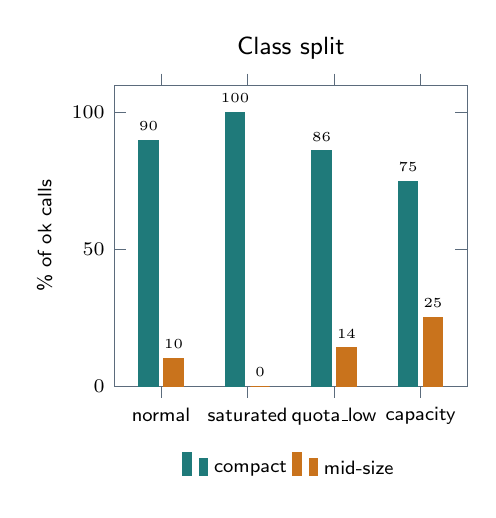
\begin{tikzpicture}
\begin{axis}[
  ybar, bar width=7pt, width=0.5\linewidth, height=5.4cm, ymin=0, ymax=110,
  symbolic x coords={normal,saturated,quota\_low,capacity}, xtick=data,
  x tick label style={font=\sffamily\scriptsize}, y tick label style={font=\sffamily\scriptsize},
  ylabel={\sffamily\scriptsize \% of ok calls}, title={\sffamily\small Class split},
  legend style={font=\sffamily\scriptsize, at={(0.5,-0.2)}, anchor=north, legend columns=2, draw=none},
  nodes near coords, every node near coord/.append style={font=\sffamily\tiny},
  enlarge x limits=0.18, axis line style={slate}, major tick style={slate}]
\addplot[fill=teal, draw=teal] coordinates {(normal,90) (saturated,100) (quota\_low,86) (capacity,75)};
\addplot[fill=amber, draw=amber] coordinates {(normal,10) (saturated,0) (quota\_low,14) (capacity,25)};
\legend{compact, mid-size}
\end{axis}
\end{tikzpicture}\hspace{2mm}%
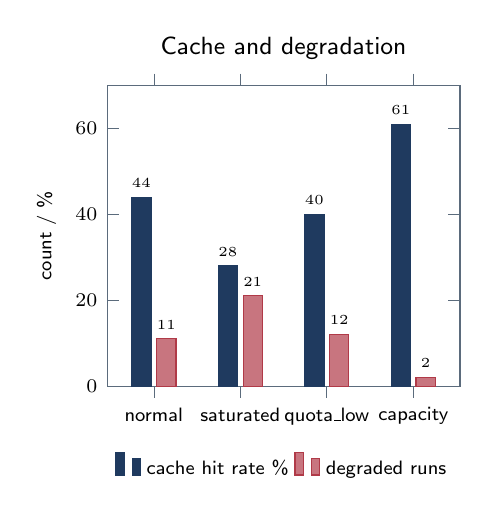
\begin{tikzpicture}
\begin{axis}[
  ybar, bar width=7pt, width=0.5\linewidth, height=5.4cm, ymin=0, ymax=70,
  symbolic x coords={normal,saturated,quota\_low,capacity}, xtick=data,
  x tick label style={font=\sffamily\scriptsize}, y tick label style={font=\sffamily\scriptsize},
  ylabel={\sffamily\scriptsize count / \%}, title={\sffamily\small Cache and degradation},
  legend style={font=\sffamily\scriptsize, at={(0.5,-0.2)}, anchor=north, legend columns=2, draw=none},
  nodes near coords, every node near coord/.append style={font=\sffamily\tiny},
  enlarge x limits=0.18, axis line style={slate}, major tick style={slate}]
\addplot[fill=navy, draw=navy] coordinates {(normal,44) (saturated,28) (quota\_low,40) (capacity,61)};
\addplot[fill=rose!70, draw=rose] coordinates {(normal,11) (saturated,21) (quota\_low,12) (capacity,2)};
\legend{cache hit rate \%, degraded runs}
\end{axis}
\end{tikzpicture}
\caption{\texttt{reports/load-engine-v1.md}. 0 exceptions reached the caller in any profile; all 7 quota refusals in \textit{quota\_low} were handled by waiting the stated delay.}
\label{fig:load}
\end{figure}

\begin{table}[H]
\centering\small
\begin{tabular}{@{}l r r r r@{}}
\toprule
& \textbf{normal} & \textbf{saturated} & \textbf{quota\_low} & \textbf{capacity}\\
\midrule
engine calls & 50 & 50 & 50 & 69\\
provider requests (all attempts / ok) & 28 / 21 & 35 / 21 & 33 / 21 & 27 / 24\\
refused attempts & 7 & 14 & 12 & 3\\
explain served in fast mode / generated & 11 / 10 & 21 / 0 & 12 / 9 & 1 / 10\\
breaker trips & 1 & 1 & 1 & 1\\
input tokens per ok call & 455 & 427 & 470 & 619\\
repeated identical provider requests & 0 & 0 & 0 & 1 → 0$^*$\\
\bottomrule
\end{tabular}
\caption{Load test details. $^*$the one repeat was a degraded explain re-sent; fixed by the negative cache (replay test; a live rerun had 0 repeats).}
\end{table}

\textbf{Capacity.} A learner turn costs 1.73 engine calls, and \textbf{2.00 provider requests when nothing
is cached}. At 20 requests/min per key that is about 20 active learners sending one message every 2
minutes, 10 at one per minute. Locally the binding limit is concurrency, not quota (11.5 s mean latency
→ 10.4 req/min); on FelCloud (v1.1, see below) the quota binds instead.

\subsection{The same measurements on FelCloud (engine v1.1, 26 Oct)}

Real provider, simulator off (\texttt{reports/felcloud-capacity-quality-2026-10-26.md}); the local column is the table above (Ollama behind the simulator). The capacity run is 40 learner turns at about 15 engine calls/min.

\begin{table}[H]
\centering\small
\begin{tabularx}{\linewidth}{@{}L{5.6cm} Y Y@{}}
\toprule
& \textbf{local v1 (Ollama)} & \textbf{FelCloud v1.1}\\
\midrule
engine calls per turn & 1.73 & 1.73\\
provider requests per turn, observed & 0.68 & 0.57\\
provider requests per \emph{cold} turn & 2.00 & 1.77\\
cache hit rate (small question pool) & 61\,\% & 62\,\%\\
mean provider latency & 11.5 s & 5.4 s\\
binding limit & concurrency, 10.4 req/min & quota, 20 req/min (concurrency ceiling 22.3)\\
cold-turn latency p50 / p95 & n/a & 10.3 / 16.6 s\\
active learners, 1 message / 2 min (cold) & 20 (quota), 10 (at local latency) & 23\\
active learners, 1 message / min (cold) & 10 & 11\\
refusals, degraded runs, exceptions & 3, 2, 0 & 0, 0, 0\\
\bottomrule
\end{tabularx}
\caption{Capacity. Plan on the cold-turn rows: the cache rate comes from a 14-message pool. The quota binds only slightly, so a slower mid-size model moves the limit back to concurrency.}
\end{table}

\begin{table}[H]
\centering\small
\begin{tabularx}{\linewidth}{@{}L{5.6cm} Y Y@{}}
\toprule
\textbf{Explain quality} & \textbf{local (Ollama 8B, 91 answers)} & \textbf{FelCloud llama3.1-8b, 35 answers}\\
\midrule
new examples & 10 (11\,\%) & 3 (9\,\%)\\
wrong\_math & 1 & 1\\
ungrounded\_formula & 2 & 3 (one also wrong\_math)\\
loop guard & 2/50 (4\,\%) & 4/35 (11\,\%); one reproduced false positive\\
language drift, contamination, truncated output & n/a & 0, 0, 0\\
output tokens / latency & n/a & mean 110 tokens; p50 9.3 s, p95 12.2 s\\
\bottomrule
\end{tabularx}
\caption{Of the flagged formulas: 2 real model errors (wrong power rule, an invented muddled example), 1 checker limitation (a cut span), 1 false positive ($f(0)=1$) whose answer also contains an undetected sign error. One run, temperature 0.3: differences of one or two answers are noise.}
\end{table}

\textbf{Priority and outages.} At 40 arrivals/min (n=60) the INTERACTIVE \texttt{engine.run} p95 was 26.8 s, made of limiter and queue wait rather than provider time; BACKGROUND absorbed the queueing (about 28 s in the queue against 0.8 s median for interactive). During a mid-size outage (26 Oct, about 40 minutes of timeouts) the breaker never opened on timeouts and two hung explains blocked classify calls for up to 190 s; see \texttt{reports/midsize-outage-2026-10-26.md} and the change list there.

\begin{table}[H]
\centering\small
\begin{tabularx}{\linewidth}{@{}L{6.2cm} Y@{}}
\toprule
\textbf{Evaluation} & \textbf{Result}\\
\midrule
classify, llama3.2:3b, 15 messages & intent 87\,\%, language 93\,\%, p50 2.6 s; manual set 4/4\\
retrieval (BM25), 15 + 4 off-topic & hit@1 13/15, hit@3 14/15, off-topic 4/4 rejected\\
cross-language (Darija/Arabizi → French docs) & hit@1 0/8 without glossary → 6/8 with it\\
explain formula check, 91 answers & 10 with new examples (correct), wrong\_math 1, ungrounded 2\\
explain loops, 50 answers & loop rate 4\,\% (2/50), salvage 1/2\\
\bottomrule
\end{tabularx}
\caption{Quality evals (\texttt{scripts/eval\_classify.py}, \texttt{eval\_retrieval.py}, \texttt{eval\_explain.py}). The glossary and its test questions were written by the same team: 6/8 is an upper bound until real learner questions are collected.}
\end{table}

% ================================================================== 14
\section{Configuration reference}
\label{sec:config}

All settings come from the environment through \texttt{config.py}; code never names a model, a URL or a
key. Defaults below are the code defaults (\texttt{.env.example} documents the same values).

\small
\begin{longtable}{@{}>{\ttfamily\raggedright\arraybackslash}p{4.9cm} >{\ttfamily\raggedright\arraybackslash}p{3.9cm} >{\raggedright\arraybackslash}p{6.4cm}@{}}
\toprule
\textrm{\textbf{Variable}} & \textrm{\textbf{Default}} & \textbf{Meaning}\\
\midrule
\endhead
\multicolumn{3}{@{}l}{\textbf{\color{navy}Provider and models}}\\
LLM\_BASE\_URL, LLM\_API\_KEY & required & OpenAI-compatible endpoint and key (never logged)\\
MODEL\_COMPACT, MODEL\_MIDSIZE & required & comma list = in-class preference order\\
MODEL\_EMBED & empty & embedding model (only for \texttt{RETRIEVER=embedding})\\
MODELS\_WITHOUT\_JSON\_MODE & empty & models that break on \texttt{response\_format}\\
REQUEST\_TIMEOUT\_S & 85 & FelCloud's server timeout is 90 s\\
\multicolumn{3}{@{}l}{\textbf{\color{navy}Platform limits (client side)}}\\
RATE\_LIMIT\_PER\_MIN, RATE\_WINDOW\_S & 20, 60 & chat sliding window: at most 20 sends in any 60 s\\
RATE\_WINDOW\_SLACK\_S & 0.5 & a send frees its slot this long after the window\\
EMBED\_RATE\_LIMIT\_PER\_MIN, EMBED\_RATE\_WINDOW\_S & 60, 60 & embeddings window (separate quota)\\
RATE\_BURST, EMBED\_BURST & 20, 60 & deprecated (simulator bucket only)\\
MAX\_CONCURRENT & 2 & requests in flight\\
BACKGROUND\_RESERVE & 6 & BACKGROUND chat waits while fewer than this many sends remain in the window (v1.3)\\
MIDSIZE\_MAX\_SLOTS, VISION\_MAX\_SLOTS & 1, 1 & slots each slow class may hold; together they leave one slot to compact (v1.2, v1.3)\\
MODEL\_VISION & deepseek-ocr & the vision class (v1.3)\\
TIMEOUT\_VISION\_S & 40 & vision request timeout; under the server's 90 s\\
VISION\_MAX\_PIXELS, VISION\_MAX\_BYTES & 1000000, 12000000 & images are resized to this many pixels; larger files are refused\\
IMAGE\_TOKENS\_PER\_MEGAPIXEL & 1000 & input tokens counted per megapixel of image (an assumption until measured)\\
MAX\_TOKENS\_VISION, OCR\_MAX\_TOKENS & 700, 700 & output caps for the vision class and the OCR task\\
CHECK\_CLAIM\_MAX\_TOKENS, CHECK\_ANSWER\_MAX\_TOKENS & 120, 80 & per-task output caps\\
COURSES\_DIR & data/courses & course graphs (units, concepts, prerequisites)\\
RAG\_COURSE\_INDEX\_DIR & data/index/courses & runtime material (uploads, professor documents), one file per course\\
SOURCE\_BOOST\_PROFESSOR & 1.3 & BM25 score factor of professor material (before the coverage gate)\\
INGEST\_MAX\_OCR\_PAGES & 20 & scanned pages read per file\\
PASSAGE\_BUDGET\_SHARE, BOARD\_BUDGET\_SHARE & 0.25, 0.25 & share of the prompt budget for explain's \texttt{passage} / \texttt{board\_text}\\
RETRIEVAL\_QUERY\_CHARS & 400 & a passage or board text is cut to this many characters as a search query\\
PREP\_LEARN\_MINUTES, PREP\_REVIEW\_MINUTES, PREP\_ASSESSMENT\_MAX & 20, 8, 10 & prep plan: planned minutes per page, assessment size\\
MAX\_TOKENS\_COMPACT, MAX\_TOKENS\_MIDSIZE & 300, 550 & output caps per class\\
OUTPUT\_CAP\_MODE & both & \texttt{options} (\texttt{options.num\_predict}), \texttt{max\_tokens} or both; FelCloud honours only \texttt{num\_predict}\\
INPUT\_TOKEN\_BUDGET & 2800 & estimated input cap enforced before sending\\
ESTIMATE\_CHARS\_PER\_TOKEN & 2.3 & token estimator (worst measured case, Arabizi)\\
CONTEXT\_WINDOW, CONTEXT\_FILL & 4096, 0.85 & estimated prompt + output cap must fit window × fill\\
INPUT\_TRUNCATION\_CHARS\_PER\_TOKEN & 5 & \texttt{prompt\_tokens} below chars/this = input cut (\texttt{input\_truncated}); 0 = off\\
BUDGET\_SAFETY\_MARGIN & 0.1 & prompts assembled within budget × (1 − margin)\\
\multicolumn{3}{@{}l}{\textbf{\color{navy}Retry and routing}}\\
MAX\_ATTEMPTS & 4 & attempts per request\\
MAX\_RETRY\_WAIT\_S & 30 & INTERACTIVE: longest stated quota delay it waits for, else degraded with an eta\\
MAX\_RETRY\_WAIT\_S\_BACKGROUND & 65 & BACKGROUND: the observed quota delay is 60 s\\
CONCURRENCY\_RETRY\_WAIT\_S & 2 & cap on a concurrency 429's wait (it states 60 s)\\
SATURATION\_RETRIES & 1 & mid-size retries before fallback\\
COMPACT\_MAX\_RETRIES & 3 & compact retries (no fallback exists)\\
QUOTA\_LOW\_THRESHOLD & 2 & local tokens below this → explain goes to fast mode\\
BREAKER\_THRESHOLD, \_WINDOW\_S, \_COOLDOWN\_S & 3, 60, 30 & mid-size circuit breaker\\
\multicolumn{3}{@{}l}{\textbf{\color{navy}Cache and prompts}}\\
CACHE\_PATH & data/\allowbreak{}cache.sqlite & SQLite file (\texttt{:memory:} in tests)\\
CACHE\_TTL\_DAYS & 7 & exact-cache lifetime\\
NEGATIVE\_CACHE\_TTL\_S & 600 & negative markers; 0 = off\\
PROMPTS\_DIR & prompts & versioned prompt files\\
\multicolumn{3}{@{}l}{\textbf{\color{navy}Retrieval and content}}\\
RETRIEVER & bm25 & \texttt{bm25} or \texttt{embedding}\\
DOCS\_DIR, RAG\_INDEX\_PATH & data/\allowbreak{}docs, data/\allowbreak{}index/\allowbreak{}chunks.json & course material and its index\\
RAG\_TOP\_K & 2 & chunks per explain after the gate\\
RAG\_MIN\_COVERAGE & 0.4 & relevance gate\\
CHUNK\_MAX\_TOKENS & 300 & chunk size\\
GLOSSARY\_PATH, GLOSSARY\_WEIGHT & data/\allowbreak{}glossary.yaml, 0.5 & learner terms → course terms (empty = off)\\
TERMS\_AR\_PATH & data/\allowbreak{}terms\_ar.yaml & Arabic math terms for MSA answers\\
EXERCISES\_PATH & data/\allowbreak{}exercises/\allowbreak{}derivees.yaml & exercise bank\\
TEMPLATES\_PATH & data/\allowbreak{}templates.yaml & openers, practice lines, feedback\\
EXPLAIN\_MAX\_TOKENS & 350 & explain output cap\\
CLASSIFY\_, HINT\_, GRADE\_, COMPRESS\_, QUIZ\_INTRO\_, FRAMING\_MAX\_TOKENS & 50, 80, 120, 30, 60, 40 & per-task output caps (cut text is trimmed to the last sentence)\\
EXPLAIN\_FREQUENCY\_PENALTY & 0.3 & discourages loops; dropped automatically if rejected\\
\multicolumn{3}{@{}l}{\textbf{\color{navy}Metrics and simulator}}\\
METRICS\_PATH & metrics/\allowbreak{}calls.jsonl & JSONL metrics\\
SIMULATE\_CONSTRAINTS & false & wrap the client in the simulator\\
SIM\_LATENCY\_COMPACT\_S, \_MIDSIZE\_S & 2,6 / 8,30 & added latency range per class\\
SIM\_RATE\_PER\_MIN, SIM\_BURST & 20, 20 & the simulated provider's real quota\\
SIM\_SATURATION\_PROB, SIM\_COMPACT\_\dots & 0.15, 0.0 & saturation probability per class\\
SIM\_SATURATION\_DIALECT & annex & \texttt{annex} (503) or \texttt{litellm} (429 cooldown)\\
SIM\_MAX\_TOKENS\_CEILING, SIM\_PROMPT\_TOKENS\_CEILING & 2048, 2048 & 400 above these\\
SIM\_MIDSIZE\_SLOTS, SIM\_TRANSIENT\_ERROR\_PROB, SIM\_SEED & 1, 0.0, — & mid-size capacity, random 5xx, seed\\
\bottomrule
\end{longtable}
\normalsize

\begin{note}[Simulator profiles]
\texttt{simulator/profiles.py} names five profiles used by the load test and by \texttt{/sim <name>} in the
console: \texttt{normal} (15\,\% mid-size saturation), \texttt{calm} (no saturation, no added latency),
\texttt{saturated} (90\,\% / 20\,\%), \texttt{quota\_low} (provider 10/min, burst 4) and \texttt{capacity}. The
simulator is an httpx transport that wraps the real one, so the gatekeeper parses genuine responses on
the same code path as FelCloud. Local Ollama never refuses anything: without the simulator, the
resilience code is never exercised.
\end{note}

% ================================================================== 15
\section{Customizing the engine}

\subsection{Teach a new subject (no code)}

\begin{enumerate}
  \item \textbf{Course material}: add \texttt{data/docs/<name>.<lang>.md} with the front matter and
  \texttt{\#\#} sections tagged \texttt{<!-{}- concept: id -{}->}; run \texttt{python -m scripts.index\_docs}.
  \item \textbf{Glossary}: add entries \texttt{- fr: [course term]} + \texttt{variants: [...]} in
  \texttt{data/glossary.yaml} (a variant may belong to one entry only; loading rejects duplicates).
  \item \textbf{Exercises}: add to the bank YAML (\texttt{id}, \texttt{concept}, \texttt{level}, \texttt{template\_key} +
  \texttt{expression} or \texttt{statement: \{fr, en, ar\}}, \texttt{solution}, \texttt{hints}, \texttt{common\_mistakes}). A test
  checks that every chunk's concept has at least one exercise.
  \item \textbf{Templates}: openers and lines per language in \texttt{data/templates.yaml}.
  \item Re-run \texttt{pytest -q} and \texttt{python -m scripts.eval\_retrieval}.
\end{enumerate}

\begin{lstlisting}[style=plain]
---
topic: derivative
level: beginner
language: FRENCH
title: Formules de dérivation
---
## Produit et quotient
<!-- concept: produit -->
Pour un produit de deux fonctions u et v : (u·v)' = u'·v + u·v'. Ce n'est pas u'·v'. ...
\end{lstlisting}

\subsection{Change a prompt}

Prompts live in \texttt{prompts/<task>.md}: a front matter with \texttt{task} and \texttt{version}, then
\texttt{\#\# name} sections (\texttt{system}, \texttt{user}, \texttt{lang.FRENCH}, \texttt{example.ARABIZI},
\texttt{fallback.DARIJA}\dots) with \texttt{\$placeholders} (Python \texttt{string.Template}). \textbf{Bump the
version} when you change the meaning: it is part of the cache key, so old answers are invalidated
without a manual flush. Re-run the relevant eval script afterwards: small models are sensitive even to
the order of few-shot examples.

\subsection{Add your own task}
\label{sec:custom-task}

A task is a \texttt{TaskSpec} plus a row in \texttt{ROUTES} plus a prompt file. \texttt{summary} already has its
routing row (compact) but no implementation, so here is a complete one. This exact code was run
against a fake provider while writing this guide: one compact request, the repeat came from the cache.

\begin{lstlisting}
# prompts/summary.md
# ---
# task: summary
# version: 1
# ---
# ## system
# Summarize the text for a $level student in at most 3 short sentences. Reply in $language.
# ## user
# $text

from engine import Engine
from engine.tasks import TaskSpec, default_registry

def summary_build(p, inputs, ctx, limit=0):
    return [{"role": "system", "content": p.render("system", level=ctx.level or "high-school",
                                                    language=(ctx.language or "FRENCH").title())},
            {"role": "user", "content": p.render("user", text=str(inputs["text"]).strip())}]

SUMMARY = TaskSpec(name="summary", prompt="summary", max_tokens=120, temperature=0.2,
                   required_inputs=("text",), build=summary_build)

registry = default_registry()
registry.register(SUMMARY)        # "summary" already has a row in router.policy.ROUTES (compact)
engine = Engine.create(registry=registry)
# r = await engine.run("summary", {"text": "..."}, {"language": "FRENCH"})
\end{lstlisting}

\texttt{TaskSpec} hooks you can add, all optional: \texttt{output\_schema} (pydantic model → JSON mode,
validation, repair), \texttt{safe\_default}, \texttt{shortcut} (answer without the LLM), \texttt{finalize\_text} /
\texttt{finalize\_data} (guards, returning a reason), \texttt{fallback\_text}, \texttt{prepare} (adjust context),
\texttt{grounded} + \texttt{render\_grounded} (RAG), \texttt{decorate} (deterministic scaffolding),
\texttt{check\_grounding} (formula check), \texttt{local} (no model at all), \texttt{rules\_on\_hit}.
A task registered without a \texttt{ROUTES} row is refused at start-up.

\subsection{Other common changes}

\begin{tabularx}{\linewidth}{@{}L{4.6cm} Y@{}}
\toprule
\textbf{You want to\dots} & \textbf{Change}\\
\midrule
switch provider or models & \texttt{.env} only (\texttt{LLM\_BASE\_URL}, \texttt{MODEL\_*}); list several models per class for failover order\\
send explain to compact always & \texttt{ROUTES["explain"] = Route(C)}, in \texttt{router/policy.py} only\\
add a model class (e.g. code) & \texttt{ModelClass} in \texttt{config.py} + \texttt{MODEL\_<CLASS>} + routes using it\\
adapt to a new error shape & \texttt{classify\_response} / header constants in \texttt{gatekeeper/errors.py}\\
store metrics elsewhere & pass \texttt{sink=} any object with \texttt{write(CallRecord)}\\
tune fallback eagerness & \texttt{QUOTA\_LOW\_THRESHOLD}, \texttt{SATURATION\_RETRIES}, \texttt{BREAKER\_*}\\
make explain shorter/longer & \texttt{EXPLAIN\_MAX\_TOKENS} + the ``≤ 120 words'' line in \texttt{prompts/explain.md}\\
expose it over HTTP & wrap \texttt{engine.run} in your web framework, one \texttt{Engine} per process (see below)\\
\bottomrule
\end{tabularx}

\begin{warn}[One engine per process, one process per key]
The rate limiter, queue, breaker and in-flight coalescing live in memory. Two worker processes
sharing one API key would each believe they have 20 requests/min. Run a single engine process per key
(behind your web server), or move the limiter state to a shared store first (§\ref{sec:improve}).
\end{warn}

% ================================================================== 16
\section{Known limitations and improvement ideas}
\label{sec:improve}

\begin{tabularx}{\linewidth}{@{}L{6.2cm} Y@{}}
\toprule
\textbf{Limitation} & \textbf{Idea}\\
\midrule
in-memory limiter/queue/breaker & a Redis-backed sliding window and breaker for multi-process deployments\\
no semantic cache (no embedding model on FelCloud) & add it for explain once an embedding model exists; keep the key on language + level + style; threshold 0.94\\
quota-exhausted shape unconfirmed & confirm in a FelCloud slot; one-line change in \texttt{errors.py}\\
local latency ≠ FelCloud & rerun \texttt{load\_test} and capacity in a FelCloud slot\\
Darija generation is weak & body stays French; templates need a native Tunisian review\\
lexical retrieval misses (e.g. ``x(x+1)'' never says ``produit'') & glossary entries from real learner questions; hybrid BM25 + embeddings\\
one topic in the bank, French statements for hints and solutions & more banks; translate hints and feedback\\
azi-1 (Arabizi ``I don't understand'') still labelled DIAGNOSTIC & handled by the confusion override; a larger eval set before tuning\\
saturated-profile priority inversion unexplained & rerun with larger n\\
SQLite calls are synchronous inside async code & fine at this scale; move to \texttt{aiosqlite} if the cache grows\\
\bottomrule
\end{tabularx}

% ================================================================== A
\appendix
\section{File map}

\begin{tabularx}{\linewidth}{@{}T{5.0cm} Y@{}}
\toprule
\textrm{\textbf{Path}} & \textbf{Contents}\\
\midrule
config.py & \texttt{Settings}, \texttt{ModelClass}, \texttt{load\_settings} (all env variables)\\
engine/core.py & \texttt{Engine}: \texttt{create}, \texttt{run}, cache/negative/coalescing, fast mode, generation, outcomes\\
engine/tasks.py & \texttt{TaskSpec}, \texttt{Registry}, the six tasks, guards, loop detection\\
engine/result.py & \texttt{Result}, \texttt{Event}\\
engine/grounding.py, mathcheck.py & formula extraction and checks; safe sympy parsing\\
engine/exercises.py, language.py, prompts.py & bank, language rules, prompt loader\\
engine/answers.py, claims.py, prep.py, course.py, vision.py & check\_answer logic, check\_claim formulas, prep plan and page exercises, course graph, image preparation (v1.3)\\
engine/fake.py & \texttt{FakeEngine}: canned realistic results for the UIs, no LLM (v1.3)\\
rag/ingest.py & PDF / DOCX / Markdown $\to$ chunks, concept tags, OCR of scanned pages (v1.3)\\
docs/ENGINE\_API.md & the integration contract, generated from real outputs (v1.3)\\
data/courses/ & course graphs (v1.3)\\
router/policy.py, breaker.py & routing table, decisions, follow-up; circuit breaker\\
gatekeeper/ & client, errors, limiter, queue, retry, cache\\
rag/ & normalize, chunker, store, glossary, retriever (BM25, embedding), budget\\
metrics/ & \texttt{CallRecord}, JSONL and memory sinks\\
simulator/ & constraint transport, profiles\\
prompts/ & classify, hint, explain, grade, compress, quiz, ocr\_transcribe, check\_claim, check\_answer (versioned)\\
data/ & docs, index, glossary, exercises, templates, Arabic terms\\
scripts/ & smoke, chat, load\_test, metrics\_report, eval\_*, index\_docs, recon\\
tests/ & 768 unit tests + 5 integration tests (\texttt{-m integration})\\
DECISIONS.md & every non-obvious design choice, with evidence\\
\bottomrule
\end{tabularx}

\end{document}
